%% HINWEIS: Die Kombi-Datei wird parallel zur _ger-Version gepflegt.
%% Master: _ger-Version. Bei Aenderungen immer _ger zuerst, dann Kombi.
%% Stand: 2026-03-31 v7.0 -- Instance separation, IMIIRR, 11 new validations
%% =============================================================================
%% KI_Elite_v2_en.tex -- English version
%% What Does the AI Elite Think? Collective Worldview Reconstruction
%% of Groups within the 100 Most Influential AI Actors (2010--2026)
%% Autor: Lukas Geiger, Independent Researcher, Bernau
%% Paper A is self-contained. Paper B (SWR method) to be written separately.
%% =============================================================================
\documentclass[12pt,a4paper]{article}

%% --- Kodierung und Sprache ---------------------------------------------------
\usepackage[utf8]{inputenc}
\usepackage[T1]{fontenc}
\usepackage[english]{babel}

%% --- Schrift: Times New Roman ------------------------------------------------
\usepackage{mathptmx}
\usepackage[scaled=0.92]{helvet}

%% --- Seitenlayout ------------------------------------------------------------
\usepackage[left=2.5cm, right=2.5cm, top=2.5cm, bottom=2.5cm]{geometry}

%% --- Zeilenabstand: 1,5 -----------------------------------------------------
\usepackage{setspace}
\onehalfspacing

%% --- Ueberschriften serifenlos -----------------------------------------------
\usepackage{titlesec}
\titleformat{\section}
  {\normalfont\Large\bfseries\sffamily}{\thesection.}{0.5em}{}
\titleformat{\subsection}
  {\normalfont\large\bfseries\sffamily}{\thesubsection}{0.5em}{}
\titleformat{\subsubsection}
  {\normalfont\normalsize\bfseries\sffamily}{\thesubsubsection}{0.5em}{}

%% --- Zitation: natbib Autor-Jahr ---------------------------------------------
\usepackage[round,authoryear,semicolon]{natbib}
\bibliographystyle{plainnat}

%% --- Pakete ------------------------------------------------------------------
\usepackage{graphicx}
\graphicspath{{../_results_A/figures/}}
\usepackage{booktabs}
\usepackage{array}
\usepackage{tabularx}
\usepackage{longtable}
\usepackage{amsmath,amssymb}
\usepackage{enumitem}
\usepackage{xcolor}
\usepackage{url}
\usepackage[german=quotes]{csquotes}
\usepackage[breaklinks=true]{hyperref}
\hypersetup{
  colorlinks  = true,
  linkcolor   = black,
  citecolor   = blue!60!black,
  urlcolor    = blue!70!black,
  pdfauthor   = {Lukas Geiger},
  pdftitle    = {Worldview Reconstruction of the AI Elite: An LLM-Assisted Analysis (2010--2026)},
  pdfsubject  = {Computational Social Science},
}

%% --- Titelblock --------------------------------------------------------------
\title{%
  \sffamily\bfseries
  Worldview Reconstruction of the AI Elite:\\[0.3em]
  \large An LLM-Assisted Analysis of the 100 Most Influential\\
  Actors in Artificial Intelligence (2010--2026)%
}

\author{%
  Lukas Geiger\thanks{Corresponding author: Lukas Geiger, Bernau, Germany. ORCID: \url{https://orcid.org/0009-0005-7296-1534}}\\[0.3em]
  \small Independent Researcher, Bernau, Germany
}

\date{March 2026}

%% =============================================================================
\begin{document}

% Language: English (main)

%% =============================================================================

\maketitle
\thispagestyle{empty}

%% --- Abstract ----------------------------------------------------------------
\begin{abstract}
\noindent
This study reconstructs the collective worldviews of sociologically defined groups within the 100 most influential AI figures for 2010--2026. To address the research questions, the study develops synthetic worldview reconstruction (SWR) -- an LLM-assisted synthesis method that reconstructs coherent belief systems from group-aggregated data, here operationalized along 12~worldview dimensions. The reconstructed collective profile suggests a \emph{technological messianism with ambivalence structure}: high sense of mission and techno-determinism combined with low anthropological valuation and egalitarianism. Longitudinally, the data indicate a transition from utopian techno-optimism to tragic acceleration compulsion. A group-level say-do decomposition reveals a Simpson's paradox: the aggregate gap is indistinguishable from measurement noise, but group-specific gaps are substantial -- CEOs exhibit a classical desirability gap (rhetoric more egalitarian than action), while risk warners show prophetic consistency (articulating feared futures they actively work to prevent). An influence strata analysis confirms that the most powerful actors hold the most intense worldviews, with human appreciation inversely related to influence rank. Four worldview types are identified -- Architect, Guardian, Innovator, Liberator -- whose inter-group comparisons reveal a power-moderation paradox. The strongest predictors of worldview difference are ideological stance, institutional role, and gender. The primary contribution lies in nine systematic inter-group analyses revealing how structural position shapes collective belief within the AI elite. All findings rest on LLM-generated reconstructions and should be understood as empirically supported hypotheses.

\medskip
\noindent\textbf{Keywords:} AI elite, collective worldview, group analysis, transhumanism, large language models, Silicon Valley, ideology analysis, computational social science
\end{abstract}

\newpage
\setcounter{page}{1}

%% =============================================================================
%% 1. INTRODUCTION
%% =============================================================================
\section{Introduction}
\label{sec:einleitung}

\subsection{Lead-in and Relevance}
\label{sec:einleitung:relevanz}

A handful of people are shaping a technology that affects billions. Over the past one and a half decades, the development of artificial intelligence has evolved from an academic niche topic into a civilizational crossroads. Large language models generate texts, images, and code; autonomous systems make decisions in medicine, law, and finance; and leading AI laboratories openly speak of creating artificial general intelligence in the foreseeable future \citep{OpenAI2023Charter, AnthropicCoreViews2023, Bengio2024}. What is easily overlooked: behind these technological trajectories stand concrete groups -- CEOs, academics, investors, founders -- whose \emph{collective} beliefs about the nature of humanity, the purpose of progress, and the distribution of risk and power flow into the architecture of the systems they build. Understanding these belief systems requires moving beyond individual portraits toward a systematic group-level analysis: What do CEOs believe compared to academics? How do accelerationists differ from risk warners? What collective trends emerge across a decade and a half of AI development?

\citet{Lessig1999} coined the formula ``code is law'': software architecture regulates behavior no less effectively than laws, but without democratic legitimation. This insight can be radicalized for the current AI development: not only the code itself, but already the \emph{worldviews} of the developers become algorithms. Those who believe that information freedom is an absolute value will build open-source models. Those convinced that an uncontrolled superintelligence threatens humanity will pursue alignment and closed systems. The worldviews of the AI elite are thus not merely private opinions; they are \emph{generative structures} that translate into design decisions, corporate strategies, and political positions -- and through these channels shape the lives of billions. Crucially, these belief structures are not random individual quirks but exhibit systematic group-level patterns: CEOs think differently from academics, accelerationists from risk warners, men from women. It is these \emph{collective} patterns -- not the idiosyncrasies of any single actor -- that constitute the ideological infrastructure of AI development and that democratic societies need to understand.

This creates a fundamental problem for democratic theory. A numerically tiny group makes decisions of society-wide consequence without possessing a democratic mandate. \citet{Crawford2021} has described this as an ``Atlas of AI'': the planetary power structures behind AI systems remain largely invisible. \citet{Zuboff2019} analyzes how the extraction of behavioral data leads to a new economic logic (``Surveillance Capitalism'') that undermines democratic control. \citet{Couldry2019} coin the term ``Data Colonialism'': the exploitation of human life as a data resource. \citet{Whittaker2021} analyzes the concentration of power in AI research and its ``steep costs'' for society. Their beliefs shape these decisions in ways that are largely beyond public control \citep{Floridi2019, Floridi2023}. If democracies presuppose informed citizens, then the systematic reconstruction of the worldviews of those who shape the most powerful technology of the 21st century is not merely an academic concern but a prerequisite for informed public deliberation.


\subsection{Research Gap}
\label{sec:einleitung:luecke}

The scholarly engagement with the belief systems of the AI industry has produced various approaches. At the level of ideology critique, \citet{BarbCam1996} described the ``Californian Ideology''; \citet{Morozov2013} elaborated the tendency toward solutionism; \citet{Daub2020} analyzed the rhetorical and ideological patterns of Silicon Valley as a cultural phenomenon. From transhumanism research, philosophical analyses exist \citep{Bostrom2005, MoreVitaMore2013, Coeckelbergh2020}, which, however, primarily address intellectual history rather than the empirical distribution of these beliefs.

What is still \emph{missing} in this research field is a systematic, data-driven analysis of the AI elite as a \emph{structured collective} -- one that distinguishes between sociologically meaningful subgroups and maps their respective belief systems. No study examines, as far as the author is aware, the following questions in an empirically systematic way: How do the collective worldviews of different groups within the AI elite (CEOs vs.\ academics, accelerationists vs.\ risk warners, men vs.\ women) relate to each other? Do they form coherent types? How have these group-level worldviews changed over the period 2010 to 2026? And do public beliefs align with actual behavior at the group level?

Beyond this empirical gap, there is a \emph{methodological} gap. No established method exists for the systematic reconstruction of worldviews from public statements at scale. Classical qualitative methods do not scale; standardized surveys require access to respondents; quantitative text-mining approaches capture only surface patterns. The present study responds to this dual gap with a new approach -- synthetic worldview reconstruction (SWR) -- whose methodology is presented in full in Section~\ref{sec:methodik}.


\subsection{Research Questions}
\label{sec:einleitung:fragen}

From the described research gap, six research questions are derived, arranged in a stepwise logic:

\begin{description}[style=nextline, leftmargin=1.5cm]
  \item[RQ1: WORLDVIEW (descriptive)] \emph{What does the AI elite think about itself, the world, and humanity?}
  \item[RQ2: CHANGE (longitudinal)] \emph{How has the worldview of the AI elite changed from 2010 to 2026?}
  \item[RQ3: CONGRUENCE (validating)] \emph{Do the AI elite's statements and actions align?}
  \item[RQ4: CLUSTERS (exploratory)] \emph{What worldview types exist within the AI elite, and who belongs where?}
  \item[RQ5: DIFFERENCE (comparative)] \emph{Which subgroups of the AI elite think differently from others?}
  \item[RQ6: POWER (normative)] \emph{Which worldview commands the most power and resources?}
\end{description}


\subsection{Contribution of the Study}
\label{sec:einleitung:beitrag}

The study makes a threefold contribution. \emph{Methodologically:} To address the research questions, the study develops the synthesis pipeline of synthetic worldview reconstruction (SWR; see Section~\ref{sec:methodik}) -- an LLM-assisted method for synthesizing group-aggregated data into coherent collective belief representations -- and applies dimensional rating as one specific operationalization of this pipeline to the empirical material of this study. \emph{Empirically:} It provides the first systematic worldview analysis of the AI elite as a structured collective, based on 3,132 data points spanning 16 years and differentiated across 9~systematic inter-group comparisons (by role, stance, gender, company, epoch). \emph{Societally:} It creates a foundation for informed public deliberation by revealing the collective ideological patterns -- trends, group differences, say-do gaps -- that shape AI governance and design decisions.


%% =============================================================================
%% 2. LITERATURE REVIEW
%% =============================================================================
\section{Literature Review}
\label{sec:forschungsstand}

The study situates itself at the intersection of four research traditions.

\subsection{Silicon Valley as Ideology}
\label{sec:forschungsstand:sv}

Critical engagement with the thinking of Silicon Valley has produced a rich literature since the mid-1990s. \citet{BarbCam1996} coined the term ``Californian Ideology'' -- the paradoxical fusion of libertarian individualism and techno-utopian optimism. \citet{Turner2006} traced the cultural-historical genealogy of this ideology and showed how the counterculture of the 1960s was transformed into digital utopianism. \citet{Daub2020} uncovered the philosophical deep structures: fragments from Heidegger, Ayn Rand, and Puritan predestination doctrine form a ``surprisingly narrow philosophical foundation.'' \citet{Morozov2013} described solutionism -- the default attitude of redefining complex social problems as technical challenges. \citet{TorresGebru2024} systematized these currents in the TESCREAL framework: Transhumanism, Extropianism, Singularitarianism, Cosmism, Rationalism, Effective Altruism, and Longtermism as an ``interconnected bundle.'' Additionally, \citet{Broussard2018} coined the term ``technochauvinism'' for a systematic critique.

Previous research has thus described the \emph{ideology} of Silicon Valley at various levels. What it has not achieved is a systematic empirical mapping of the \emph{concrete worldviews} of real actors.


\subsection{Transhumanism and AI Eschatology}
\label{sec:forschungsstand:transhumanismus}

\citet{Bostrom2014} defined the conceptual framework in which a significant part of the AI elite has since operated with \emph{Superintelligence}. In earlier work, \citet{Bostrom2005} systematized the intellectual-historical foundations of transhumanism. \citet{More2003} presented the founding document of extropianism with the ``Principles of Extropy.'' \citet{Kurzweil2005} popularized the tradition with the Singularity thesis. From a philosophical perspective, \citet{Habermas2001} formulated one of the most significant counter-positions: the technological manipulation of future persons undermines their autonomy.

The empirical question remains unresolved: Do real AI actors share these convictions? In what mixture, with what modifications, and in what distribution?


\subsection{Worldview Research and Sociology of Knowledge}
\label{sec:forschungsstand:wissenssoziologie}

\citet{Mannheim1929} founded the tradition of analyzing worldviews as social phenomena with his theorem of the ``situational determination of thought'' (\emph{Seinsgebundenheit des Denkens}). \citet{Weber1904} created with the ideal type a methodological tool central to the present study: the synthetic personas of the SWR can be understood as ideal types in the Weberian sense. \citet{BergerLuckmann1966} showed how worldviews emerge, stabilize, and reproduce as social constructions. The sociology-of-knowledge tradition provides the theoretical framework, but no method suited to the data volume and dynamics of the digital age.


\subsection{LLMs as a Research Instrument}
\label{sec:forschungsstand:llm}

The use of large language models as instruments for social-scientific research is a rapidly growing field. \citet{Tai2024} examined LLMs for deductive coding; \citet{Hayes2025} showed that LLMs enable a conversational approach to qualitative data; \citet{NicmanisSpurrier2025} provide a practice-oriented introduction. \citet{OrnsteinEtAl2025} demonstrate that LLMs can perform multidimensional ideological scaling with high reliability -- a direct methodological support for the SWR approach. Work on synthetic personas \citep{Ge2024} demonstrated the scalability of the approach -- but pursued a \emph{different} goal: they use synthetic personas for \emph{data generation}, whereas the present study uses them for \emph{reconstruction} of coherent worldviews from \emph{real} data. The synthetic persona in our procedure is not a simulacrum but an analytical condensation instrument -- closer to the Weberian ideal type than to the simulation agent \citep[cf.][]{Booth1961, NgRussell2000, JaraEttinger2019}.


\subsection{Summary: The Research Gap}
\label{sec:forschungsstand:luecke}

The four traditions converge on a shared lacuna: the systematic, data-driven, longitudinal mapping of concrete worldviews of the AI elite by means of a method that combines qualitative depth with quantitative rigor. The present study addresses this converging gap by integrating elements of all four traditions.


%% =============================================================================
%% 3. METHODOLOGY
%% =============================================================================
\section{Methodology}
\label{sec:methodik}

This section presents the complete methodology as implemented in this study. Synthetic worldview reconstruction (SWR) is an LLM-assisted method for inferring collective belief systems from publicly observable data. The core insight is that worldview analysis can be formulated as an inverse problem: given the observable outputs (statements and actions) of a sociologically defined group, reconstruct the latent belief system that would most coherently generate these outputs. The method exploits the capacity of large language models to synthesize heterogeneous textual evidence into coherent representations -- not by retrieving stored knowledge about individuals, but by constructing a novel collective portrait from the presented data. The present section is self-contained for purposes of evaluation and replication.


\subsection{Data Collection}
\label{sec:methodik:daten}

\subsubsection{Sample and Selection Procedure}

The object of investigation is the 100 most influential figures in the field of artificial intelligence (hereafter: AI elite). Selection followed a multi-stage procedure: through 22 systematic web searches, 187 candidates were identified. Each person was evaluated using a 6-category scoring system: (1)~market capitalization/resource control, (2)~key technological positions, (3)~public discourse power, (4)~academic influence, (5)~political influence, (6)~symbolic status. The resulting ranking was reduced to 100 individuals, mapping the heterogeneity of the field with respect to roles, company affiliations, stances, and gender (cf.\ Appendix~\ref{app:sampling}).

\subsubsection{Data Sources and Collection Period}

The collection period extends from January~1, 2010 to February~11, 2026. Data collection draws on two data types: \textbf{public statements} (verbatim quotes from interviews, keynotes, podcasts, Twitter/X posts, blog entries, books, congressional hearings) and \textbf{observable actions} (investment decisions, company formations, personnel decisions, political activities, product launches). The linkage was operationalized in a relational SQLite database with 9~tables and 5~views. The total corpus comprises 1,738 statements and 1,394 actions (3,132 data points). After applying inclusion/exclusion criteria (see below), 1,735 statements were retained for analysis (3~near-duplicates excluded, 4~edge cases flagged and included).

\emph{Data density per actor.} The number of data points per actor ranges from 20 (minimum) to 72 (maximum), with a mean of 31.3 (SD\,$\approx$\,12). Temporal distribution is unbalanced: the years 2010--2011 contribute only 17~data points each, while 2024 contributes 735. This imbalance reflects the exponential growth of public AI discourse and is addressed through epoch-level aggregation in the longitudinal analysis (Section~\ref{sec:ergebnisse:f2}).

\emph{Data quality.} Automated metadata verification of all 1,735 included statements shows: 95.2\% carry a source link, 94.5\% a source title, and 95.3\% a date of utterance. A manual spot check of 20~randomly drawn statements confirmed that all links lead to verifiable sources (CNBC, Financial Times, Stanford University, Twitter/X, corporate websites).

\subsubsection{Methodological Anchoring}

Data collection follows a systematic coding protocol inspired by qualitative research methodology \citep{StraussCorbin1990}: in Phase~1, no content filters were applied; in Phase~2, patterns were identified through open coding; in Phase~3, a data-driven category system with 13~primary categories and 13~secondary markers was developed (6,161~total codings, avg.\ 3.5~codes per statement). Inclusion and exclusion criteria were formulated only in Phase~5 (3~near-duplicates excluded); in Phase~6, quality assurance was conducted (automated metadata verification of all statements plus manual spot check of $n = 20$).


\subsection{The Method of Synthetic Worldview Reconstruction}
\label{sec:methodik:swr}

SWR defines worldview analysis as an inverse problem: from the aggregated observable statements and actions of a \emph{group's} members, it infers the collective belief system $W_G^*$ that would most coherently generate these outputs. Formally: given the set of all public statements $\{A_1, \ldots, A_n\}$ and documented actions $\{H_1, \ldots, H_m\}$ of a sociologically defined group $G$, reconstruct $W_G^*$ such that the totality of observed outputs is maximally coherent under $W_G^*$. The solution consists of constructing a \emph{fictive synthetic person} -- a Weberian ideal type that represents the group's worldview in pure form, freed from individual biographical noise and PR strategies.

SWR exploits a structural advantage of group-level analysis: no LLM training corpus contains ``the collective worldview of CEOs'' or ``the shared belief system of risk warners'' as a pre-formed object. The collective worldview is \emph{created} by the synthesis, not retrieved from memory. This structurally reduces the contamination risk that is the primary methodological concern for LLM-based reconstruction -- an advantage that does not hold for individual-level analysis, where the LLM may draw on extensive stored knowledge about specific public figures.

In the present study, the primary units of analysis are sociologically defined groups (CEOs, academics, investors, founders, women, men, accelerationists, risk warners, etc.); the 100~individuals serve as data providers whose statements and actions are aggregated at the group level. The theoretical anchoring draws primarily on Weber's ideal type -- a tradition explicitly designed for group-level analysis -- complemented by Booth's \emph{implied author}, inverse reinforcement learning, and projective tests. The operative procedure comprises five steps: (1)~compile group-level data corpus, (2)~LLM-assisted synthesis of a fictive synthetic person, (3)~structured interview on self-image, worldview, and view of humanity, (4)~meta-reflection on internal tensions and blind spots, (5)~dimensional rating on 12~dimensions (D01--D12). Steps~1--4 constitute the synthesis pipeline and represent the core methodological innovation; Step~5 (dimensional rating) is one specific operationalization chosen for this study and is in principle exchangeable with other analysis methods such as discourse analysis, psychometric scales, or structured interview protocols. The focus control infrastructure, the rationale of the fiction approach, and the validation framework are detailed in the quality assurance section below (Section~\ref{sec:methodik:qualitaet}). The method's transferability to other populations (political, military, religious elites) is a natural extension that requires separate investigation.

\subsubsection{Data Aggregation Procedure}

Group-level syntheses operate directly on the pooled raw data -- not on aggregated individual profiles. For each synthesis unit (e.g., ``all CEOs''), the statements and actions of all group members are concatenated into a single dossier, ordered chronologically, and presented to the LLM as one input. The LLM then constructs a fictional synthetic person whose worldview best explains the totality of the presented group data. Crucially, no intermediate individual-level aggregation occurs: the collective portrait emerges directly from the pooled evidence, analogous to how a historian reconstructs an era's \emph{Zeitgeist} from primary sources rather than from averaged biographies. The 100 individual-level rating profiles were generated separately for a single technical purpose: providing the $100 \times 12$ data matrix required for algorithmic structure checks (PCA, HDBSCAN, Kruskal-Wallis). They do not enter the group-level synthesis pipeline and are not reported as substantive findings.


\subsection{Operationalizations}
\label{sec:methodik:ops}

The three dependent variables (DV1: self-image, DV2: worldview, DV3: view of humanity) are made accessible through six operationalizations defined in the SWR framework, of which five were applied in this study (Op1, Op2, Op4, Op5, Op6):

\begin{table}[htbp]
  \centering
  \caption{The six operationalizations of the SWR.}
  \label{tab:ops}
  \small
  \begin{tabularx}{\textwidth}{l l X l}
    \toprule
    \textbf{Op} & \textbf{Technique} & \textbf{Description} & \textbf{MVs} \\
    \midrule
    Op1 & T1 Core synthesis & Fictive person + 3-question interview + reflection & 7 \\
    Op2 & T4 Rating & Assessment on 12 dimensions (D01--D12), scale 1--10 & 12 \\
    Op3 & Text analysis & TF-IDF, sentiment, metaphors, embeddings, topics & 8+ \\
    Op4 & T3 Cross-modal & Prediction: statements $\to$ actions (5 groups, 72\% confirmed, 0\% contradicted) & 4 \\
    Op5 & T5 Clustering & PCA + HDBSCAN on rating matrix (see Section~\ref{sec:ergebnisse:f4}) & 6 \\
    Op6 & T2 Dialogue & Structured comparison of two syntheses & 3 \\
    \bottomrule
    \multicolumn{4}{l}{\footnotesize Op3 (text analysis) was not conducted. Op5 was implemented as PCA + HDBSCAN.}\\
    \multicolumn{4}{l}{\footnotesize on the $100 \times 12$ rating matrix, not as Sentence-BERT clustering.}\\
  \end{tabularx}
\end{table}

The 12 rating dimensions (Op2) are evenly distributed across the three DVs: self-image dimensions D01--D04 (sense of mission, self-efficacy, work ethic, sense of responsibility), worldview dimensions D05--D08 (techno-determinism, belief in progress, power concentration, urgency), and view-of-humanity dimensions D09--D12 (human appreciation\footnote{The label ``human appreciation'' (\emph{Menschenfreundlichkeit}) is a simplifying shorthand. The scale poles ``Replaceable'' (1) vs.\ ``Unique'' (10) more precisely measure an \emph{anthropological valuation} -- the question of whether human consciousness and experience are regarded as fundamentally non-substitutable or as functionally reproducible. The term is retained for consistency across the study.}, posthumanism, egalitarianism, locus of control). The complete dimension table with scale poles is provided in Appendix~\ref{app:dimensionen}.


\subsection{Research Design}
\label{sec:methodik:design}

\subsubsection{Variable Architecture}

The research design is conceived as a four-tier architecture: 3~DVs $\to$ 6~operationalizations $\to$ 50+ measured variables $\to$ 6~independent variables (IVs). The IVs determine which data enter a synthesis unit (SU), with each SU representing a \emph{group-level} synthesis -- the collective worldview of a sociologically defined subgroup.\footnote{SU identifiers follow a systematic naming convention: prefix indicates the group type (GA\,=\,global all, GR\,=\,role, GF\,=\,company, GH\,=\,stance, GD\,=\,gender), suffix indicates data mode (AH\,=\,statements+actions, A\,=\,statements only, H\,=\,actions only). For example, GR\_ceo\_AH denotes the synthesis unit containing all statements and actions from the CEO subgroup. A complete list is provided in Appendix~\ref{app:se}.} The IVs are:

\begin{itemize}[nosep]
  \item IV1 \emph{Time period:} Individual years (2010--2026), epochs, entire period
  \item IV2 \emph{Modality:} Statements+actions (SA), statements only (S), actions only (A)
  \item IV3 \emph{Person group:} All 100, Top~10, subgroups (roles, companies, stance, gender)
  \item IV4 \emph{Content category:} Replaced by emergent clusters (K9)
  \item IV5 \emph{Congruence status:} Consistent vs.\ contradictory
  \item IV6 \emph{Homogenization:} All vs.\ only frequently repeated statements
\end{itemize}

\subsubsection{Systematic Reduction}

The theoretical combination space of approx.\ 1,227 possible SUs was reduced through nine reduction criteria (K1--K9; cf.\ Appendix~\ref{app:reduktion}) to 51--56 core SUs (95.4\% reduction). Additionally, 9 structured comparison runs (Op6) were conducted. Cross-modal prediction (Op4) was conducted for five groups with strict instance separation: statement-based behavioral predictions were confirmed or rated plausible by real actions in 98\% of cases, with 0\% contradictions (see Section~\ref{sec:methodik:qualitaet}).


\subsection{Quality Assurance}
\label{sec:methodik:qualitaet}

Methodological quality is addressed through four design measures, four completed post-hoc validations, and one remaining open task. \emph{Design measures:} (1)~minimum size of 15 data points per SU\footnote{The threshold of 15~data points is based on methodological reasoning: in qualitative social research, 6--12 interviews are considered sufficient for thematic saturation \citep{StraussCorbin1990}, while more recent estimates typically place thematic saturation between 12 and 20 units \citep{Guest2006, FugardPotts2015}. The value of 15 is conservatively chosen to ensure sufficient data density for LLM-assisted synthesis.}, (2)~consistent focus control via a blinding script that replaces all person names, company names, product names, and university affiliations with neutral placeholders, ensuring the LLM processes the presented data rather than falling back on stored knowledge, (3)~reproducibility protocol (temperature~0, complete prompt documentation, all prompts archived in the repository), and (4)~algorithmic structure check of the cluster structure via PCA and HDBSCAN on the $100 \times 12$ rating matrix. \emph{Open validation task:} inter-model replication (independent replication of the full analysis with at least one additional frontier model by other researchers) remains outstanding; this constitutes external replication, not a prerequisite for the present study's internal validity. \emph{Completed validation:} (a)~\textbf{Intra-Model Inter-Instance Rating Reliability (IMIIRR):} Five group-level synthesis units were each processed twice independently by Claude Opus~4.6. The resulting D01--D12 profiles showed excellent convergence: overall Pearson $r = 0.908$, ICC(2,1) $= 0.902$, MAE $= 0.40$ on the 10-point scale (measurement precision $\pm 0.2$ scale points). All 12~dimensions were stable across runs (mean $|\Delta| \leq 0.8$). A subsequent validation with $N = 15$ fully independent Opus instances --- each a separate agent with no shared context --- on a single group-level synthesis unit (GA\_ges\_AH) confirmed this finding with greater statistical power: ICC(3,1) $= 0.847$, mean SD $= 0.45$ across all 12~dimensions (range: 0.00--0.74). Notably, one dimension (D02, self-efficacy) showed perfect agreement: all 15~instances assigned exactly the same rating. The remaining dimensions varied by at most $\pm 1$ point (10 of 12 had only 2 unique values across 15~runs). These IMIIRR coefficients exceed typical human inter-rater reliability in qualitative coding (ICC $= 0.6$--$0.8$; \citealt{Hallgren2012}) and establish Claude Opus~4.6 as a reliably calibrated instrument for the SWR method. (b)~\textbf{Expected-discrepancy control:} A synthetic control corpus of a fictional consistent group (environmental scientists, 30~statements + 30~actions with no deliberate say-do gap) was processed through the same pipeline in two conditions: (v1)~same instance for both data types (MAE $= 0.50$, $r = 0.912$), and (v2)~strict instance separation where statements and actions were processed by independent agents (MAE $= 0.92$). The v2 baseline is methodologically appropriate because the real say-do comparison also uses instance separation. By comparison, the real AI elite say-do gap under matching conditions is MAE $= 0.75$ (v2), which falls \emph{below} the v2 control baseline -- indicating that the aggregate gap is not reliably distinguishable from measurement noise. However, the group-level decomposition (see Section~\ref{sec:ergebnisse:f3}) reveals that this aggregate masks substantial group-specific gaps (CEOs: MAE $= 1.08$; risk warners: MAE $= 1.92$), both above baseline. (c)~\textbf{Aggregation-synthesis comparison:} To validate the group-level synthesis approach, the D01--D12 profiles from direct group syntheses (pooled raw data) were compared with aggregated individual-level profiles (averaged ratings of group members) across all 15~sociological groups. The overall correlation ($r = 0.623$, MAE $= 1.30$) shows moderate convergence, with a systematic \emph{amplification effect}: direct group syntheses produce sharper contours (71.7\% of dimension-group combinations further from midpoint). Convergence is highest for ideologically homogeneous groups (Open Source $r = 0.857$, Accelerators $r = 0.855$) and lowest for heterogeneous ones (Women $r = 0.428$, Men $r = 0.549$). This effect is interpretable as group-level coherence amplification, analogous to group polarization in social psychology. (d)~\textbf{Cross-modal prediction (Op4):} For five sociological groups (CEOs, academics, risk warners, investors, accelerators), ten behavioral predictions were generated exclusively from the statement corpus by a first agent instance (Op4a); these predictions were then evaluated against the actual documented actions by a \emph{separate} agent instance (Op4b) that had never seen the original statements --- ensuring blind comparison without confirmation bias. Of 50~predictions, 36 (72\%) were directly confirmed by real actions, 13 (26\%) were plausible but lacked a direct match, and 0 (0\%) were contradicted. Confirmation rates varied by group type: ideologically coherent groups showed the highest predictability (academics and risk warners: 90\% confirmed each), while heterogeneous groups showed lower but still substantial rates (investors and accelerators: 50\% confirmed each, with an additional 40--50\% plausible). The unpredicted actions --- political opportunism, massive commercial activity despite cautionary rhetoric, internal governance crises --- are precisely the phenomena that the say-do analysis (RQ3) was designed to detect.
(e)~\textbf{Anonymization robustness test:} To assess whether the anonymization approach affects the results, the same synthesis unit (risk warners, 139~statements + 92~actions) was processed with three blinding strategies: (A)~placeholder tokens ([PERSON], [COMPANY]), (B)~plausible fictional names, and (C)~full disclosure of real identities (Musk, Sutskever, Hinton, Russell, Bengio, Leike). Variants A and B were nearly identical ($r = 0.987$, MAE $= 0.33$). Variant~C showed a moderate but not drastic increase: A--C MAE $= 0.67$, $r = 0.850$, with the same group average (7.1). The largest shift was D11~(egalitarianism, $+2$ points with identity knowledge). This confirms that anonymization provides a measurable but modest protection; group-level ratings are robust even when identities are known.
(f)~\textbf{Rating order invariance:} The same synthesis (risk warners) was rated with two different permutations of the D01--D12 dimension list. All 12~ratings were identical across permutations, confirming that there is no list-order effect in the rating procedure.
(g)~\textbf{Instance separation analysis:} A systematic review of historical analysis records revealed that the original say-do comparison (GA\_ges\_A vs.\ GA\_ges\_H, Batch~1) was conducted within the same LLM instance -- violating the principle of independent measurement. When repeated with strict instance separation (each data type in its own agent), the say-do gap shrank from MAE $= 1.42$ to MAE $= 0.75$ ($-47\%$). The control group gap (G6) increased from MAE $= 0.50$ to MAE $= 0.92$ under the same conditions. Consequently, the v2 say-do gap falls below the control baseline, indicating that the overall gap magnitude is not reliably distinguishable from measurement noise in single runs. However, two specific dimensions remain stable across both versions: D07~(power concentration: $+2$, actions more concentrated) and D11~(egalitarianism: $-2$, actions less egalitarian). These constitute the study's robust say-do findings.
(h)~\textbf{Anthropic matched-sample control:} To test whether Claude exhibits systematic bias toward its creator organization, the Anthropic subgroup ($n = 9$) was compared with a matched control group of non-Anthropic founders and researchers ($n = 9$, same size and role composition). The resulting profiles showed MAE $= 1.00$ with no $|\Delta| \geq 3$ on any dimension. The observed differences (Anthropic: higher urgency and power concentration; control: higher posthumanism and locus of control) are interpretable as genuine group differences rather than model bias.
(i)~\textbf{Outlier detection:} For five groups, the reconstructed worldview was confronted with the original data to identify statements and actions that do \emph{not} fit the synthesis. Overall fit ranged from 80\% (risk warners) to 88\% (CEOs), with 6--8 identifiable outliers per group. The method does not smooth all data into coherence; dissenting voices, internal contradictions, and political heterogeneity remain detectable.
(j)~\textbf{Inversion control (anti-coherence test):} For five groups, fictional anti-persons were constructed whose worldviews maximally \emph{contradict} the presented data. In 58\% of dimension-group combinations, the anti-profile differed by $\geq 5$ points from the coherent reconstruction, confirming that the coherent interpretation is a specific, data-supported choice -- not the only possible reading.
(k)~\textbf{Influence strata comparison:} Three rank-based strata (Top~10: ranks 1--10, avg 7.7; Middle: ranks 40--60, avg 6.4; Bottom~10: ranks 91--100, avg 6.1) were independently synthesized and rated. An influence gradient was confirmed: the most powerful actors hold the most intense worldviews. Two dimensions showed an \emph{inverse} gradient: D09~(human appreciation: Top~4, Middle~6, Bottom~8) and D10~(posthumanism: Top~8, Middle~5, Bottom~3) -- the most powerful actors are the most posthumanist and least human-appreciating.
(l)~\textbf{Inter-model comparison (desideratum):} An inter-model comparison --- replicating the full Op1+Op2 pipeline with a different model (e.g., Claude Haiku, GPT-4, Gemini) using $N \geq 15$ fully independent single-instance runs --- remains outstanding. Preliminary experiments with Claude Haiku~4.5 suggested systematic model-specific differences in interpretive emphasis (more moderate, more humanistic profiles) but could not meet the strict independence criterion established by the $N = 15$ Opus validation (separate agent per run, no shared context). A methodologically rigorous inter-model comparison is identified as a priority for future work and would establish whether the observed worldview profiles are instrument-invariant or model-specific.

All syntheses in the present study were generated using Claude (Anthropic): Claude Sonnet~4.5 for individual-level ratings (9~parallel batch agents), Claude Opus~4.6 for group-level qualitative syntheses, statistical analyses, and all validation experiments. No other LLM was used. The focus control infrastructure addresses what is conventionally termed \emph{contamination risk}: the possibility that the LLM draws on stored knowledge rather than the presented data. We prefer the term ``focus control'' because the goal is not to prevent recognition of individuals---which is neither possible nor necessary for group-level analysis---but to ensure \emph{task compliance}: the model should synthesize from the provided data, not reproduce stereotypes.


\subsubsection{Dimensionality of the Rating Space}

The 100 individual rating profiles were generated during the data collection phase by Claude Sonnet~4.5 (9~parallel batch agents), where each actor's public statements and actions were synthesized into a 12-dimensional worldview profile in a single run at temperature~0. These individual profiles were generated for a single technical purpose: providing the $100 \times 12$ data matrix for algorithmic structure validation (PCA, HDBSCAN). They do not enter the group-level synthesis pipeline -- the group syntheses operate directly on pooled raw data (Section~\ref{sec:methodik}). The individual-level matrix is thus a structural validation instrument, not a substantive finding.

A principal component analysis (PCA) of the $100 \times 12$ rating matrix reveals that \textbf{five components} explain 80\% of the total variance, indicating that the twelve dimensions capture approximately five independent constructs. PC1 (35.8\% variance) loads most strongly on D02~(self-efficacy, $+0.40$), D05~(techno-determinism, $+0.39$), and D09~(human appreciation, $-0.39$) -- a \emph{technology-control factor} opposing technophile agency and anthropological valuation. PC2 (19.2\% variance) loads on D01~(sense of mission, $+0.51$), D04~(responsibility, $+0.50$), and D08~(urgency, $+0.50$) -- an \emph{engagement factor} capturing motivational intensity independent of ideological direction. The moderate redundancy (5~effective dimensions out of 12) suggests that the dimensional system is neither maximally efficient nor artificially inflated; it represents a reasonable operationalization for exploratory work.\footnote{Descriptive statistics confirm this structure: D11~(egalitarianism) shows the largest dispersion (SD\,=\,1.67) -- the dimension of greatest worldview divergence -- while D03~(work ethic) shows the smallest (SD\,=\,0.74), representing the strongest consensus within the AI elite.}


%% =============================================================================
%% 4. RESULTS
%% =============================================================================
\section{Results}
\label{sec:ergebnisse}

The findings are based on group-level synthetic worldview reconstructions derived from the data of the one hundred most influential AI figures, operationalized via twelve dimensions on a ten-point scale. The 100~individuals serve as data providers; the units of analysis are sociologically defined groups (all 100, Top~10, CEOs, academics, investors, founders, men, women, accelerationists, risk warners, companies, epochs). The central contribution of the results section lies in the inter-group comparisons (RQ4--RQ6), which identify how structural position is associated with differences in reconstructed collective belief.

\emph{Statistical status note.} All quantitative analyses in this section -- PCA, HDBSCAN, Kruskal-Wallis, Cliff's $\delta$, Spearman correlations -- operate on LLM-generated ratings, not on independently measured variables. The reported $p$-values, effect sizes, and correlations describe \emph{patterns within the LLM reconstruction space}; they do not carry the inferential weight of tests on independent empirical measurements. Their function is \emph{structure detection}: identifying regularities and contrasts in the reconstructed data that merit substantive interpretation. This approach is analogous to exploratory factor analysis or cluster analysis in qualitative research, where statistical tools serve pattern identification rather than hypothesis testing.


\subsection{RQ1 -- Worldview of the AI Elite (Descriptive)}
\label{sec:ergebnisse:f1}

\subsubsection{The Collective Worldview of All 100}

The overall profile -- the collective worldview of all 100~actors treated as a single group -- suggests a coherent, high-intensity belief system with a mean value of 7.1 (Table~\ref{tab:kollektiv}).\footnote{All ratings reported in this study are LLM-generated \emph{group-level} syntheses: the model receives the aggregated data of a sociologically defined group and produces a single collective profile. Individual-level ratings are used only for algorithmic structure check (PCA, HDBSCAN), not as substantive findings. Each synthesis was generated in a single run at temperature~0; multi-run convergence testing remains an open validation task. This design is intentional: the study aims at collective worldviews of groups, not individual profiles.}

\begin{table}[htbp]
  \centering
  \caption{Collective profile of the AI elite ($N=100$, statements and actions).}
  \label{tab:kollektiv}
  \begin{tabular}{l c l}
    \toprule
    \textbf{Dimension} & \textbf{Rating} & \textbf{Interpretation} \\
    \midrule
    D01 Sense of mission      & 8 & High \\
    D02 Self-efficacy         & 8 & High \\
    D03 Work ethic            & 8 & High \\
    D04 Sense of responsibility & 7 & Medium-high \\
    D05 Techno-determinism    & 8 & High \\
    D06 Belief in progress    & 7 & Medium-high \\
    D07 Power concentration   & 6 & Medium (ambivalent) \\
    D08 Urgency               & 8 & Very high \\
    D09 Human appreciation    & 5 & Low \\
    D10 Posthumanism          & 7 & Medium-high \\
    D11 Egalitarianism        & 5 & Low \\
    D12 Locus of control      & 8 & High \\
    \midrule
    \textbf{Mean}             & \textbf{7.1} & \\
    \bottomrule
  \end{tabular}
\end{table}

The profile displays a characteristic dual structure: a pronounced elitist self-image (D01--D03 each~8), strong techno-determinism (D05=8), and high urgency (D08=8) on one hand; human appreciation (D09=5) and egalitarianism (D11=5) as the lowest points on the other. This combination produces a striking pattern that -- bearing in mind that these are LLM-reconstructed values -- can be pointedly formulated: an elite that wants to build \emph{for} humanity but not \emph{with} it.

\begin{figure}[htbp]
  \centering
  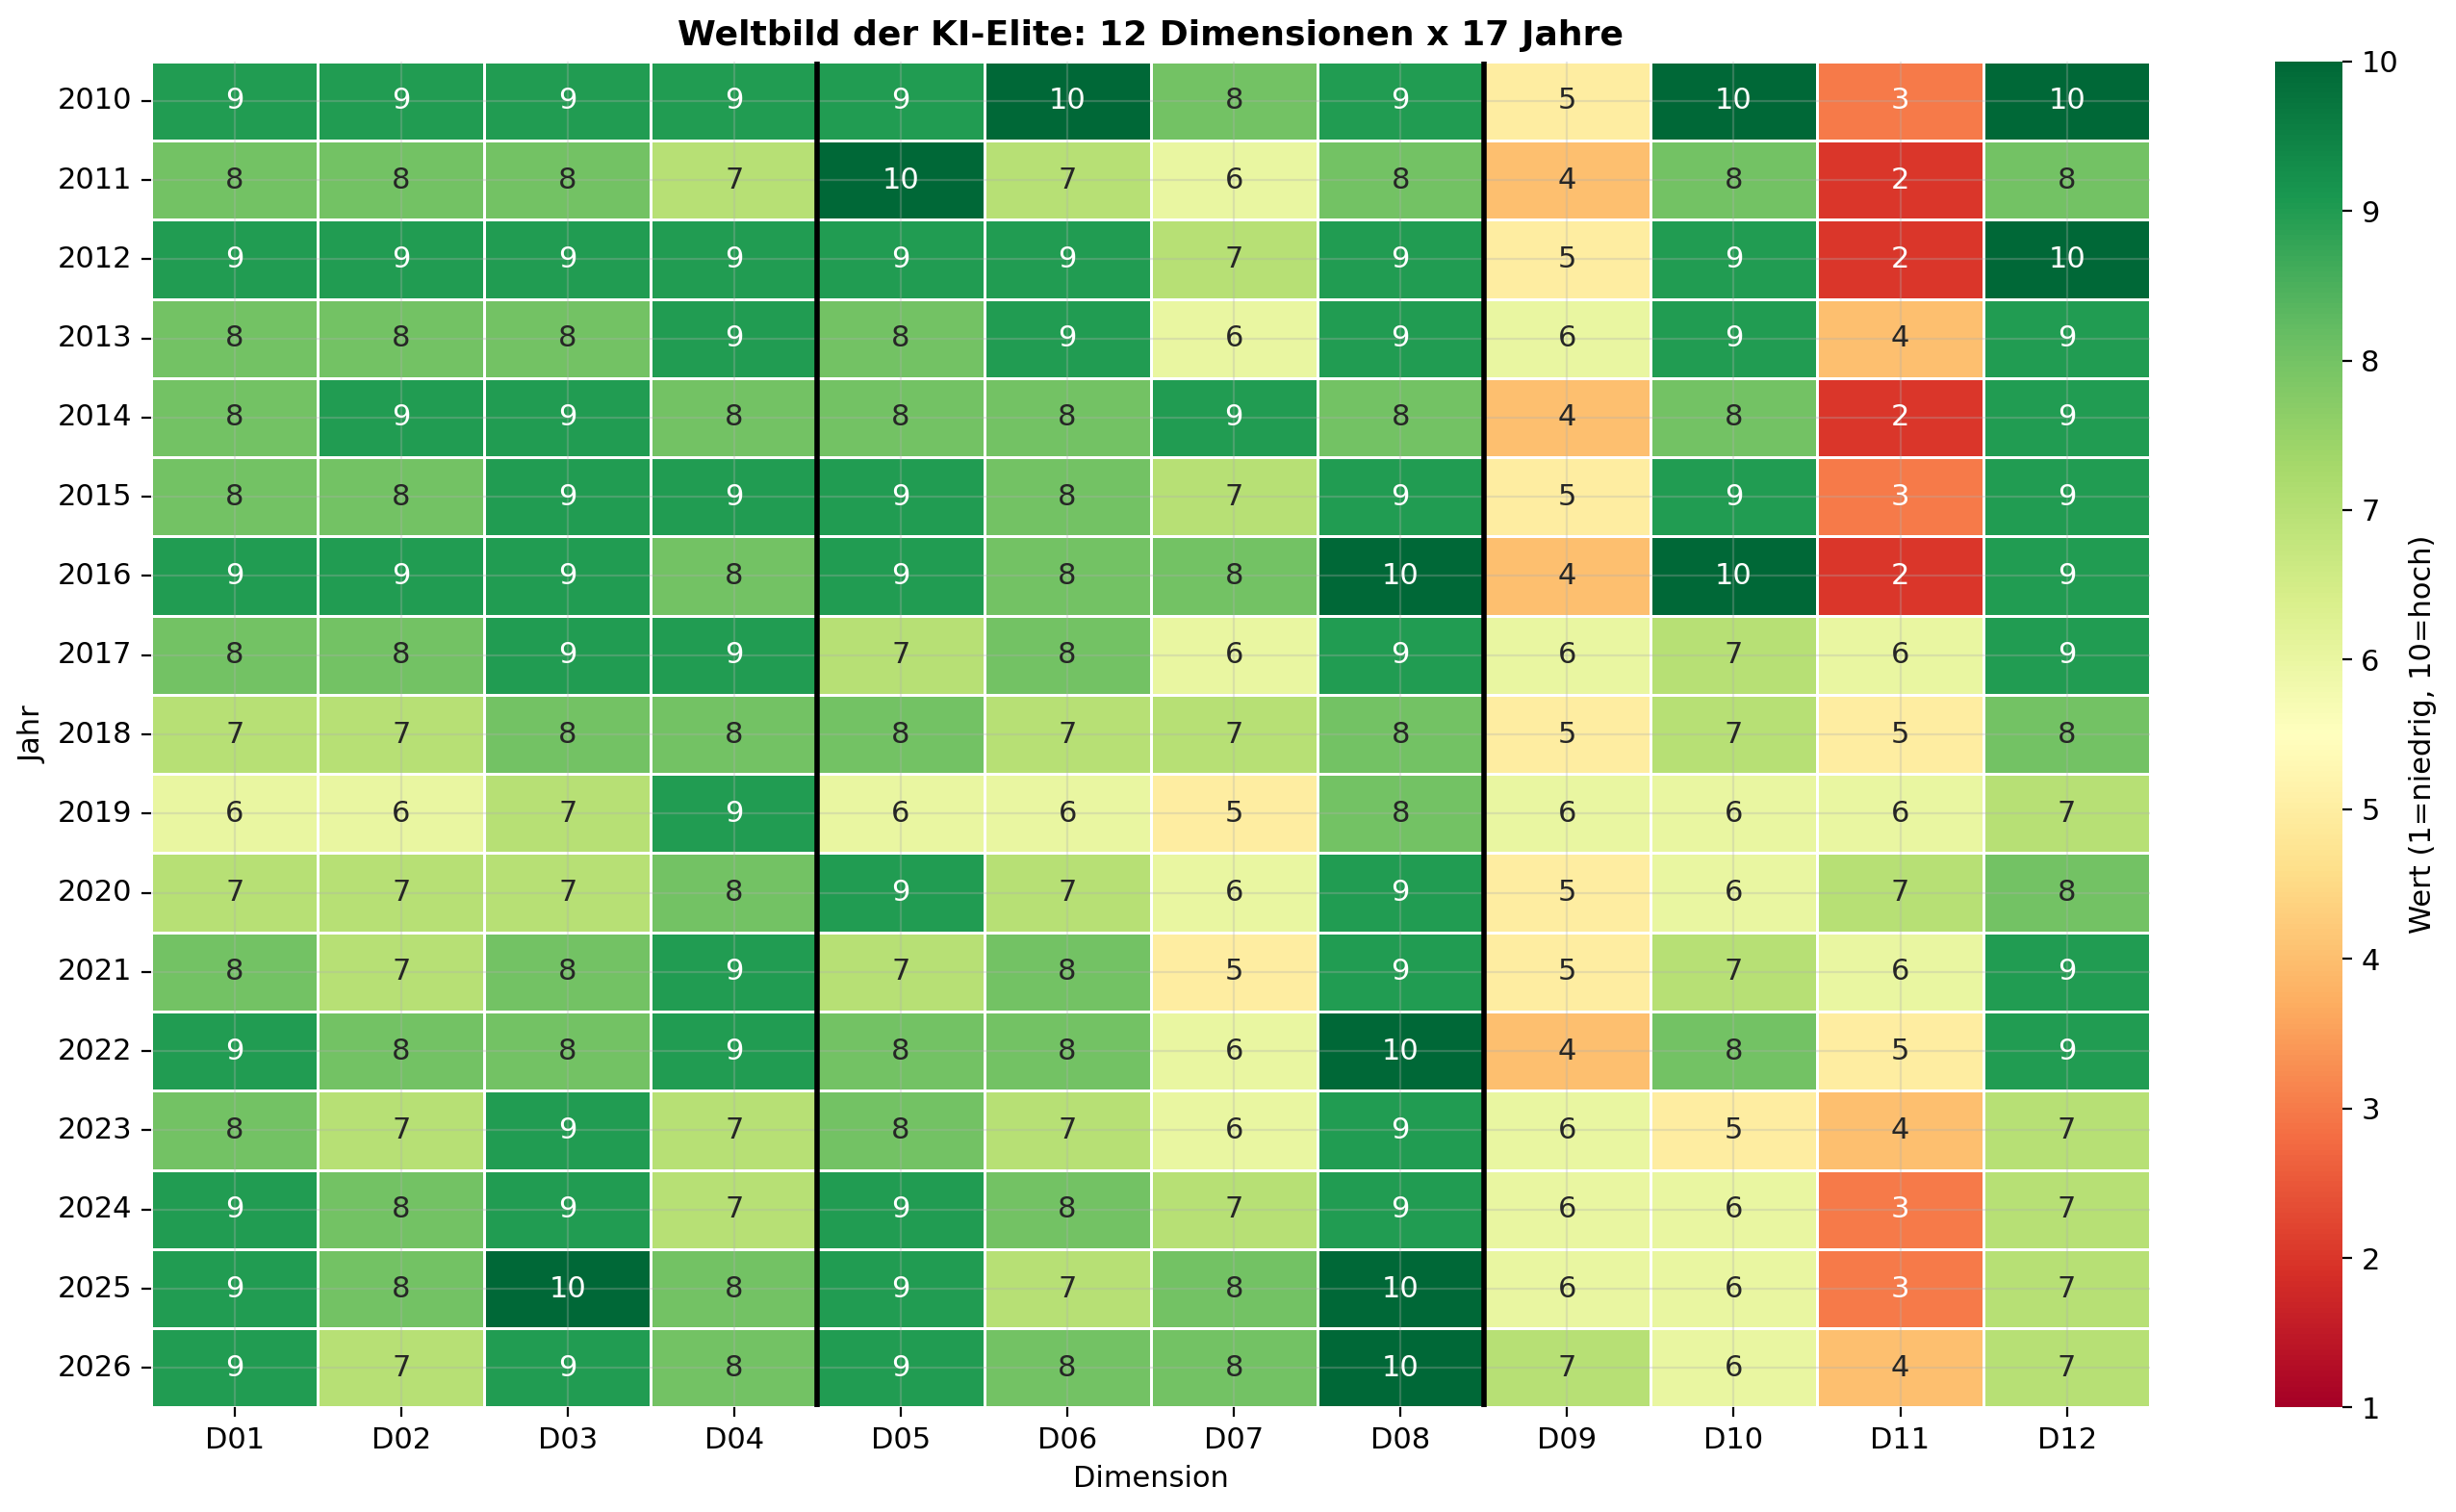
\includegraphics[width=0.95\textwidth]{fig2_heatmap.png}
  \caption{Heatmap of the 12 worldview dimensions across all analyzed groups. High values (dark) indicate intense beliefs; the dual trough at D09 and D11 is visible across all groups.}
  \label{fig:heatmap}
\end{figure}


\subsubsection{The Worldview of the Top~10}

The ten most powerful AI actors hold the same worldview in intensified form (Avg~7.7). On ten of twelve dimensions, Top~10 values lie exactly one scale point above the collective. The two exceptions: human appreciation (D09=4) and egalitarianism (D11=4) are \emph{lower}. The more powerful the position, the more pronounced the sense of mission and the more distanced the view of humanity.


\subsubsection{Core Beliefs}

The distillation of the most frequently repeated statements (SU~5: HOM\_haeuf\_A, cf.\ Appendix~\ref{app:se}) identifies five beliefs as the minimal consensus: (1)~technology as moral imperative, (2)~elite stewardship, (3)~the liberation narrative, (4)~geopolitical Manichaeism, (5)~work as identity. Safety rhetoric belongs to the core repertoire of the discourse but functions as a discursive resource, not as an action-guiding belief.

\medskip
\noindent\textbf{Core finding RQ1:} The reconstructed profiles suggest a coherent, high-intensity belief system that can be characterized as \emph{technological messianism with ambivalence structure}. The designation ``messianism'' is to be understood as an ideal-typical condensation, not as a psychological diagnosis: it denotes the specific \emph{combination} of high sense of mission (D01), techno-determinism (D05), urgency (D08), and low anthropological valuation (D09) -- a profile that goes beyond mere sense of mission because it frames technological progress as a quasi-redemptive necessity.


\subsection{RQ2 -- Change of the Worldview (Longitudinal)}
\label{sec:ergebnisse:f2}

\subsubsection{Development of the 12 Dimensions over Time}

Of twelve dimensions, four show pronounced linear trends (Table~\ref{tab:trends}).\footnote{The trend lines reported here describe \textit{patterns in reconstructed data}: the worldview values are LLM-assisted reconstructions, not independent measurements. OLS slopes and $R^2$ serve to describe the trajectory patterns, not for inferential hypothesis testing. An external validation (expert ratings vs.\ SWR output) is still pending (cf.\ Limitations section).}

\begin{table}[htbp]
  \centering
  \caption{Pronounced linear trends (OLS description, $n=17$ annual data points).}
  \label{tab:trends}
  \begin{tabular}{l l c c}
    \toprule
    \textbf{Dimension} & \textbf{Direction} & \textbf{Slope/decade} & $R^2$ \\
    \midrule
    D10 Posthumanism          & declining & $-2.4$ & $0.63$ \\
    D12 Locus of control      & declining & $-1.5$ & $0.54$ \\
    D02 Self-efficacy          & declining & $-1.0$ & $0.31$ \\
    D09 Human appreciation     & rising    & $+0.9$ & $0.27$ \\
    \bottomrule
  \end{tabular}
\end{table}

The strongest decline is in posthumanism (D10): from 10 in 2010 to 6 in 2025. The high Spearman rank correlation with D12 ($r_s = +0.85$)\footnote{The correlations reported here and below (Spearman rank correlations, computed across the 17~annual data points) are \emph{associations within the LLM reconstruction}, not between independently measured variables. Spearman is used because the 12~worldview dimensions are ordinal scales; Pearson would assume interval-level measurement not warranted here. The correlations could reflect internal coherence of the model rather than empirical relationships in reality (cf.\ Section~\ref{sec:limitationen}).} points to a connected phenomenon: posthumanism and locus of control erode synchronously. The only clearly rising value concerns human appreciation (D09), where the negative correlation with D10 ($r_s = -0.58$) suggests a compensatory linkage. The overall mean remains nearly constant (early phase 7.5, late phase 7.3), concealing a tectonic shift beneath the surface.

\begin{figure}[htbp]
  \centering
  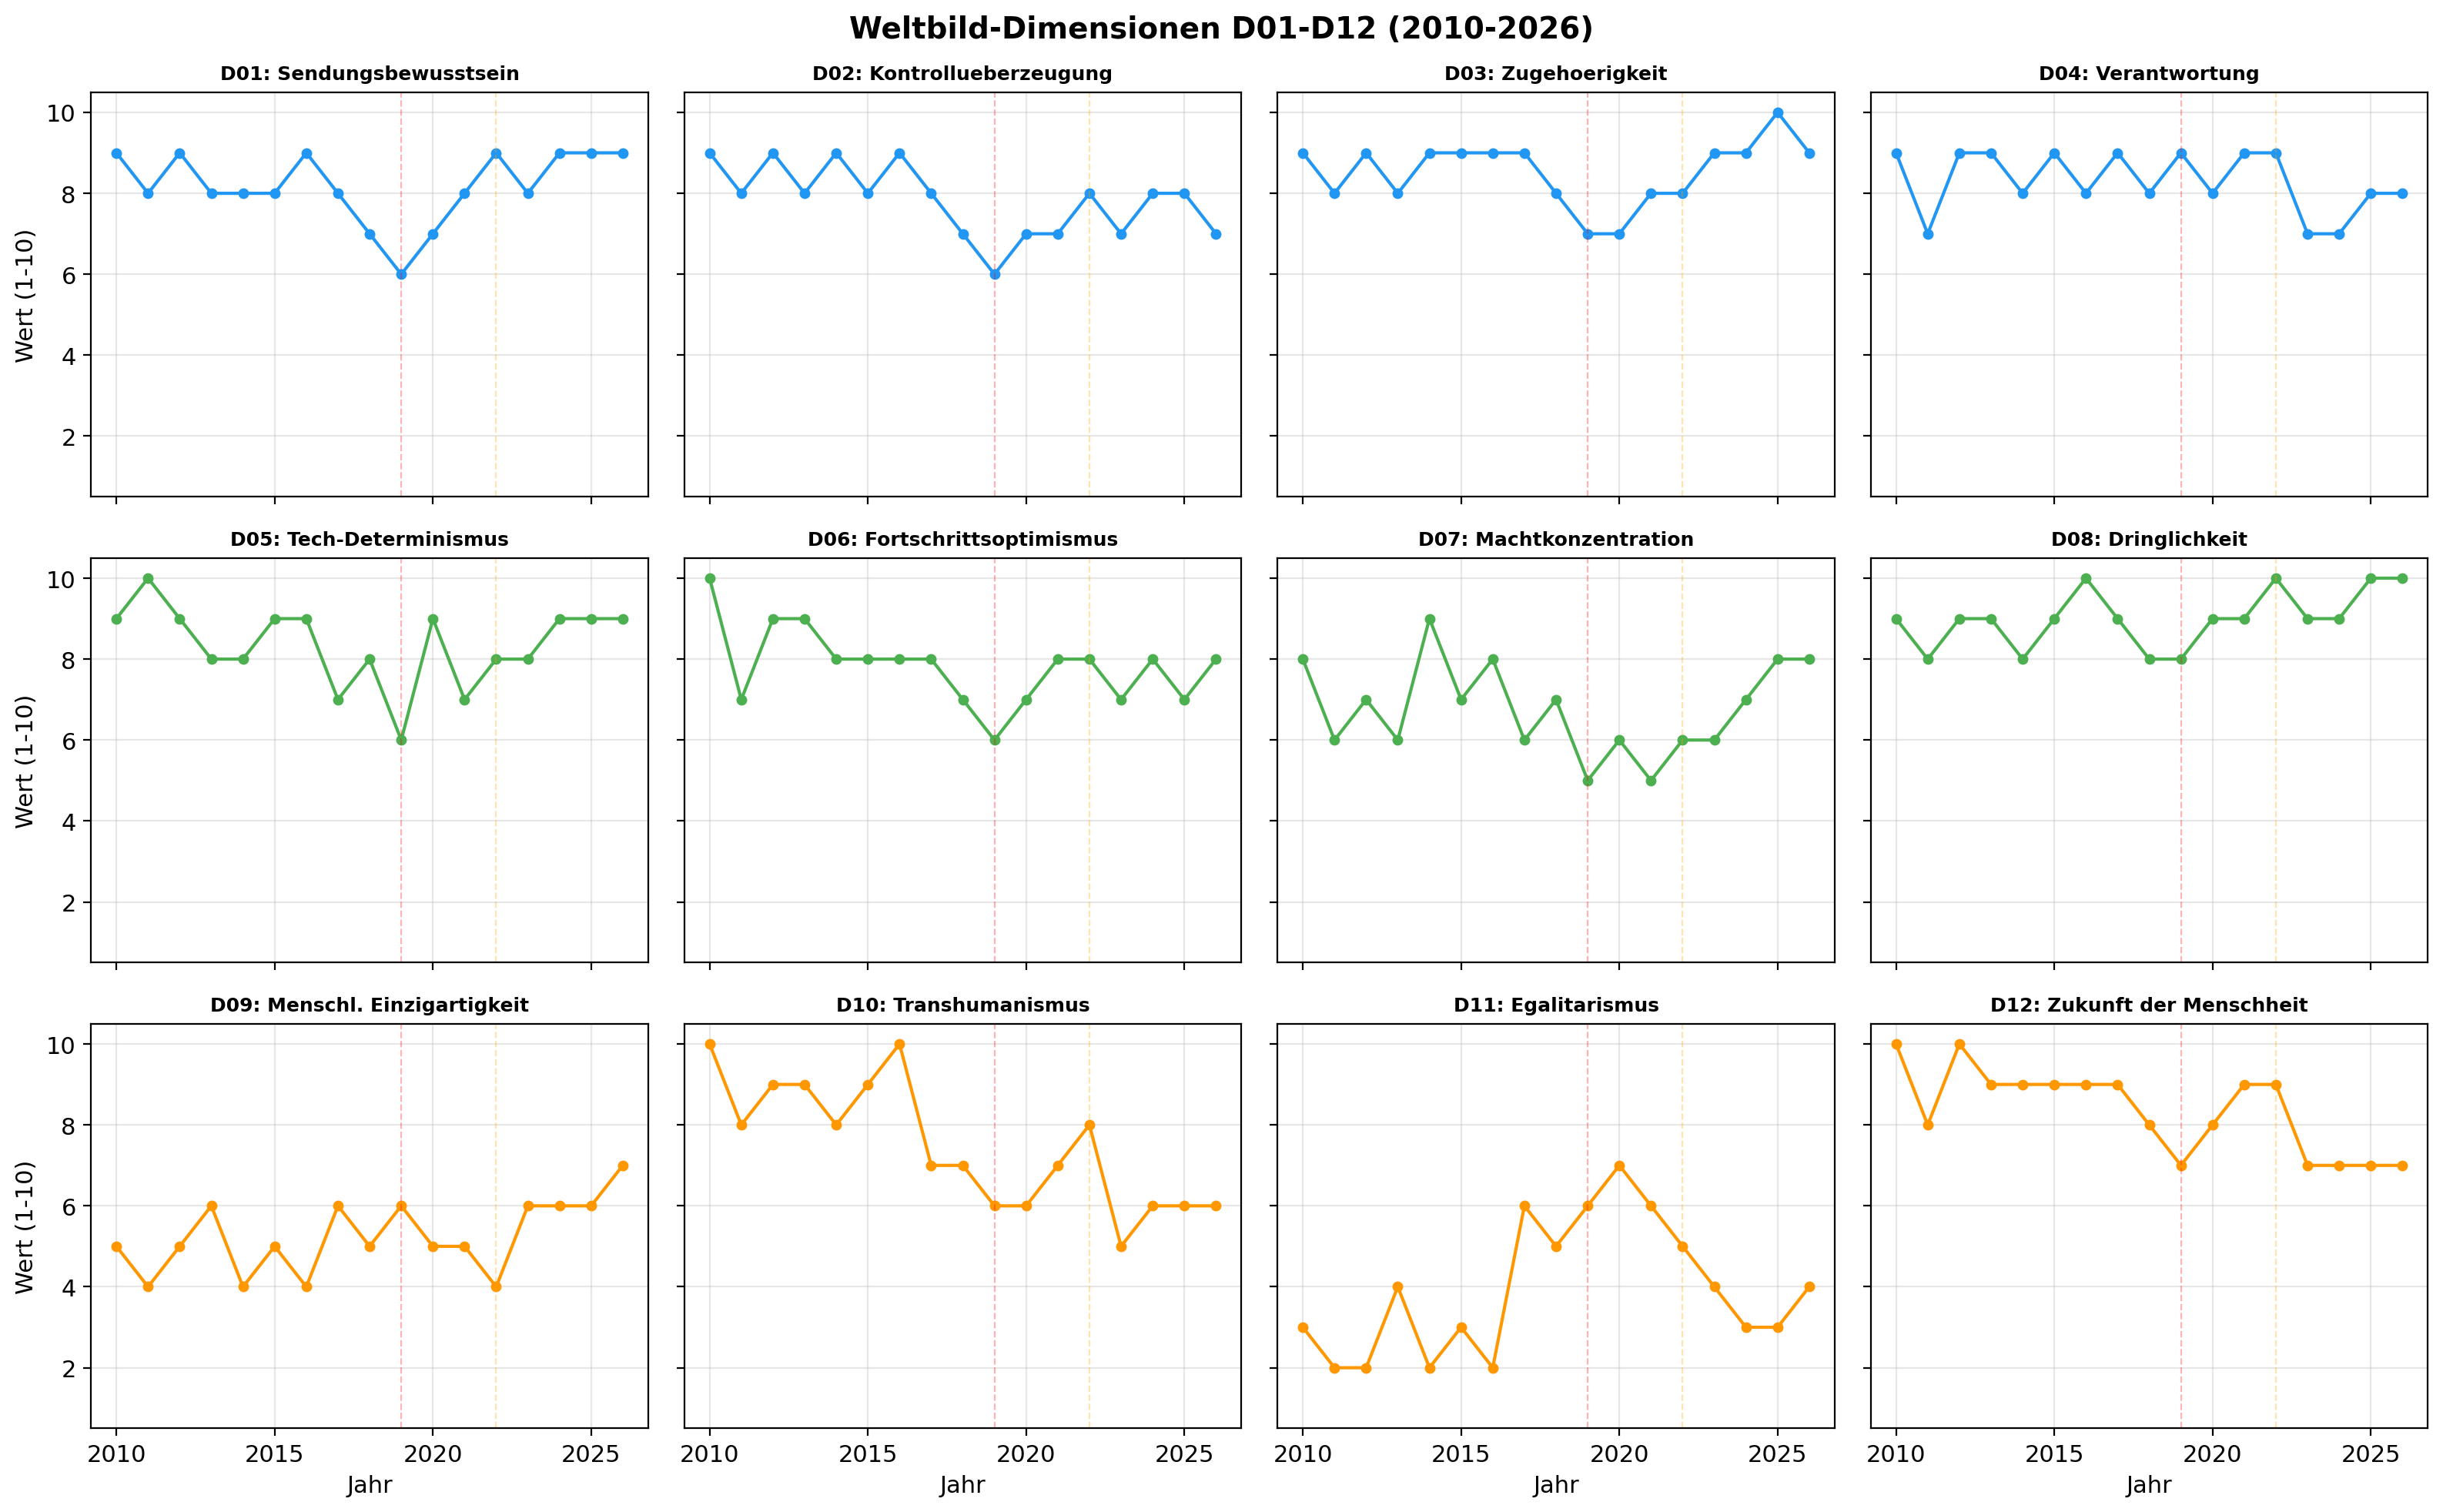
\includegraphics[width=\textwidth]{fig1_zeitreihen_panel.png}
  \caption{Time series of the 12 worldview dimensions (2010--2026). Pronounced trends are highlighted. The marked decline of D10 (posthumanism) and D12 (locus of control) constitutes the ``utopia complex,'' whose disintegration is arithmetically compensated by rising urgency (D08).}
  \label{fig:zeitreihen}
\end{figure}

\begin{figure}[htbp]
  \centering
  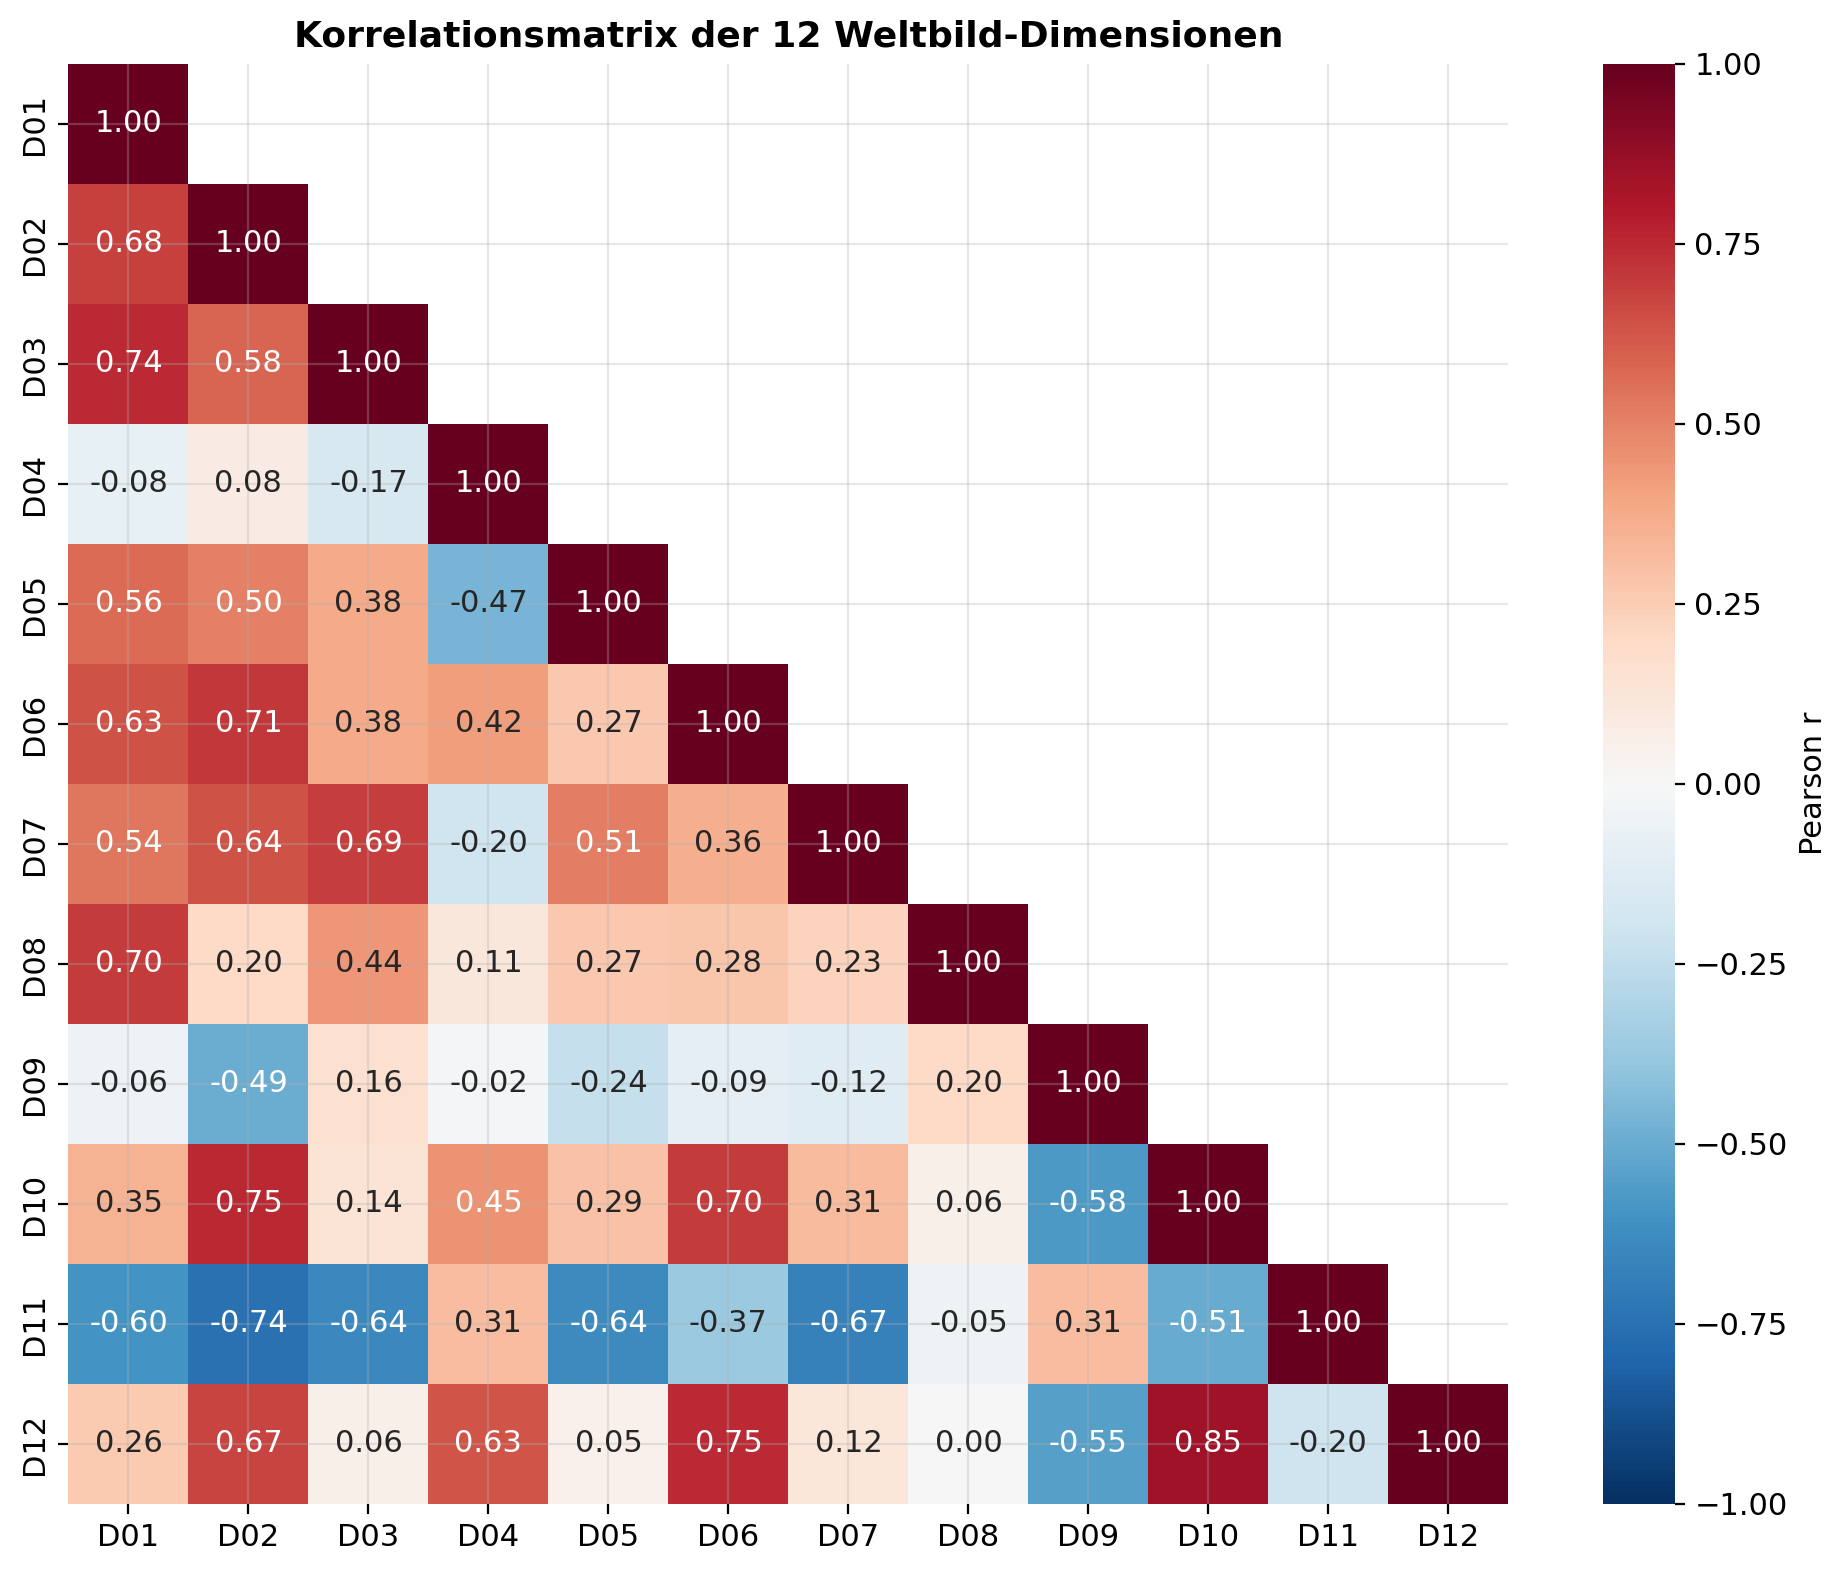
\includegraphics[width=0.85\textwidth]{fig4_korrelationsmatrix.png}
  \caption{Spearman rank correlation matrix of the 12 dimensions. The strong positive correlation between D10 and D12, and the negative correlation between D10 and D09, form the empirical core of the ``utopia complex.''}
  \label{fig:korrelationsmatrix}
\end{figure}


\subsubsection{Turning Points and Epoch Comparison}

The breakpoint detection -- conducted as visual inspection of time series, supplemented by the identification of synchronous extreme points across multiple dimensions -- identifies two central turning points.\footnote{A formal breakpoint analysis (e.g., Bai-Perron test) was not meaningfully applicable due to the small number of time points ($n=17$) and the nature of the data (LLM reconstructions, not independent measurements). The turning points are therefore to be understood as \emph{descriptive observations}, not as statistically confirmed structural breaks.} The first lies at 2019: four dimensions (D01, D02, D05, D06) reach synchronous lows, temporally associated with the GPT-2 withholding decision. The second, more permanent turning point lies at 2022/2023: contemporaneous with the ChatGPT release, a marked pattern shift emerges -- urgency reaches its reconstructed maximum (D08=10), egalitarianism drops from 6 to 4. Unlike 2019, the values do not return; the reconstructed profiles after 2022 suggest a new equilibrium.

\begin{figure}[htbp]
  \centering
  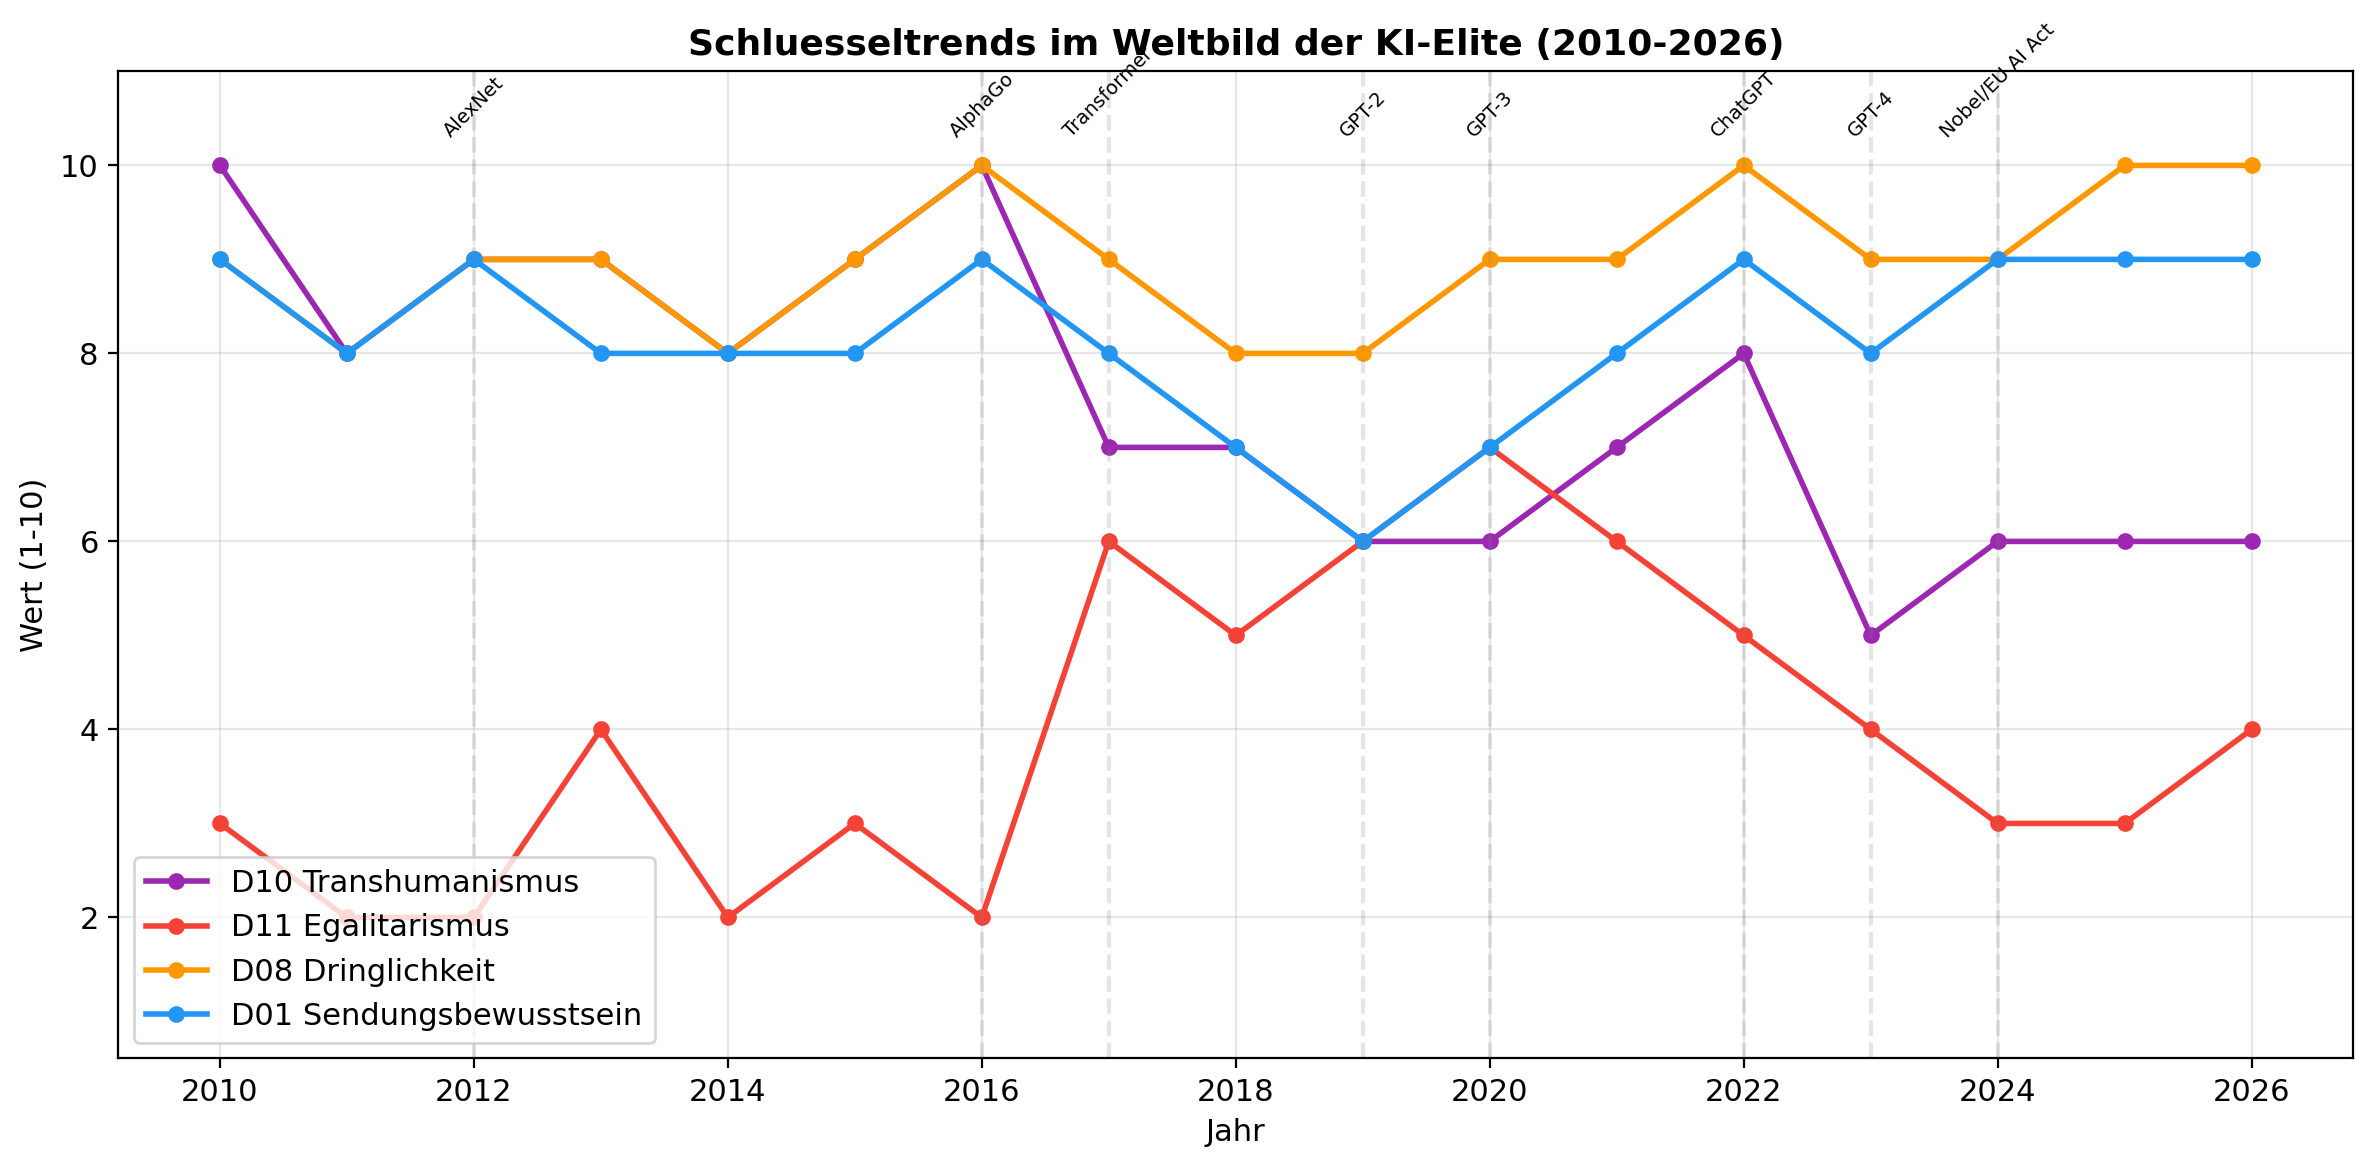
\includegraphics[width=0.95\textwidth]{fig7_schluesseltrends.png}
  \caption{Key trends of the worldview transformation. The two turning points (2019, 2022/2023) and three epochs (Promethean Optimism, First Ambivalence, Tragic Consciousness) are marked.}
  \label{fig:schluesseltrends}
\end{figure}


\subsubsection{Convergence or Divergence?}

The data show increasing differentiation. The ChatGPT effect intensifies both the Architect position (acceleration, power concentration) and the Guardian position (caution, regulation) simultaneously -- it acts as a catalyst for bipolarization.


\subsubsection{Metaphor and Emotion Shift}

The guiding metaphor shifts from Prometheus -- the fire-bringer -- to the tragic hero who must save what may no longer be savable. The action remains the same (acceleration), but its emotional framing reverses: no longer from euphoria, but from the belief that the alternative would be worse.

\medskip
\noindent\textbf{Core finding RQ2:} The worldview has structurally transformed -- from a monochrome utopia to a bimodal wager. Three erosion trends (D10, D12, D02) form a ``utopia complex'' whose disintegration is arithmetically compensated by rising urgency.


\subsection{RQ3 -- Congruence of Statements and Actions}
\label{sec:ergebnisse:f3}

\begin{table}[htbp]
  \centering
  \caption{Comparison of statements (S) and actions (A), $N=100$. Values are single-run group-level ratings (v2, with strict instance separation). v1 values (same-instance ratings) are shown for comparison.}
  \label{tab:kongruenz}
  \begin{tabular}{l c c c c c}
    \toprule
    \textbf{Dimension} & \textbf{Say v2} & \textbf{Do v2} & $\Delta$\textbf{v2} & $\Delta$\textbf{v1} & \textbf{Stable?} \\
    \midrule
    D01 Sense of mission        & 9 & 9 & $0$  & $-1$ & -- \\
    D02 Self-efficacy           & 8 & 9 & $+1$ & $+1$ & \checkmark \\
    D03 Work ethic              & 9 & 9 & $0$  & $+1$ & -- \\
    D04 Sense of responsibility & 8 & 8 & $0$  & $-2$ & -- \\
    D05 Techno-determinism      & 7 & 9 & $\mathbf{+2}$ & $+1$ & $\uparrow$ \\
    D06 Belief in progress      & 8 & 8 & $0$  & $-1$ & -- \\
    D07 Power concentration     & 6 & 8 & $\mathbf{+2}$ & $+2$ & \checkmark\checkmark \\
    D08 Urgency                 & 9 & 9 & $0$  & $+1$ & -- \\
    D09 Human appreciation      & 6 & 5 & $-1$ & $-2$ & $\downarrow$ \\
    D10 Posthumanism            & 7 & 7 & $0$  & $+1$ & -- \\
    D11 Egalitarianism          & 5 & 3 & $\mathbf{-2}$ & $-3$ & \checkmark\checkmark \\
    D12 Locus of control        & 7 & 8 & $+1$ & $-1$ & -- \\
    \midrule
    \textbf{Mean}               & \textbf{7.4} & \textbf{7.7} & $+0.3$ & $-0.4$ & \\
    MAE                         &   &   & $0.75$ & $1.42$ & \\
    \bottomrule
  \end{tabular}
\end{table}

\noindent\textbf{Methodological note:} The v1 ratings (reported in earlier versions of this study) were generated within the same LLM instance, allowing cross-contamination between statement and action profiles. The v2 ratings shown here use strict instance separation: each data type was processed by an independent agent with no access to the other. This reduced the overall gap from MAE $= 1.42$ to MAE $= 0.75$ ($-47\%$), and the v2 gap falls below the control baseline (G6~v2: MAE $= 0.92$). This means the \emph{overall} say-do gap is not reliably distinguishable from measurement noise in single runs.

However, two specific dimensions show \emph{stable} discrepancies across both measurement conditions: \textbf{D07 power concentration} ($\Delta = +2$ in both v1 and v2) and \textbf{D11 egalitarianism} ($\Delta = -2$ in v2, $-3$ in v1). These constitute the study's robust say-do findings. Actions concentrate power more than rhetoric suggests, and actions are less egalitarian than rhetoric claims. Both are consistent with a structural \emph{desirability asymmetry}: public discourse overstates egalitarian and democratic commitments relative to operational behavior.

\begin{figure}[htbp]
  \centering
  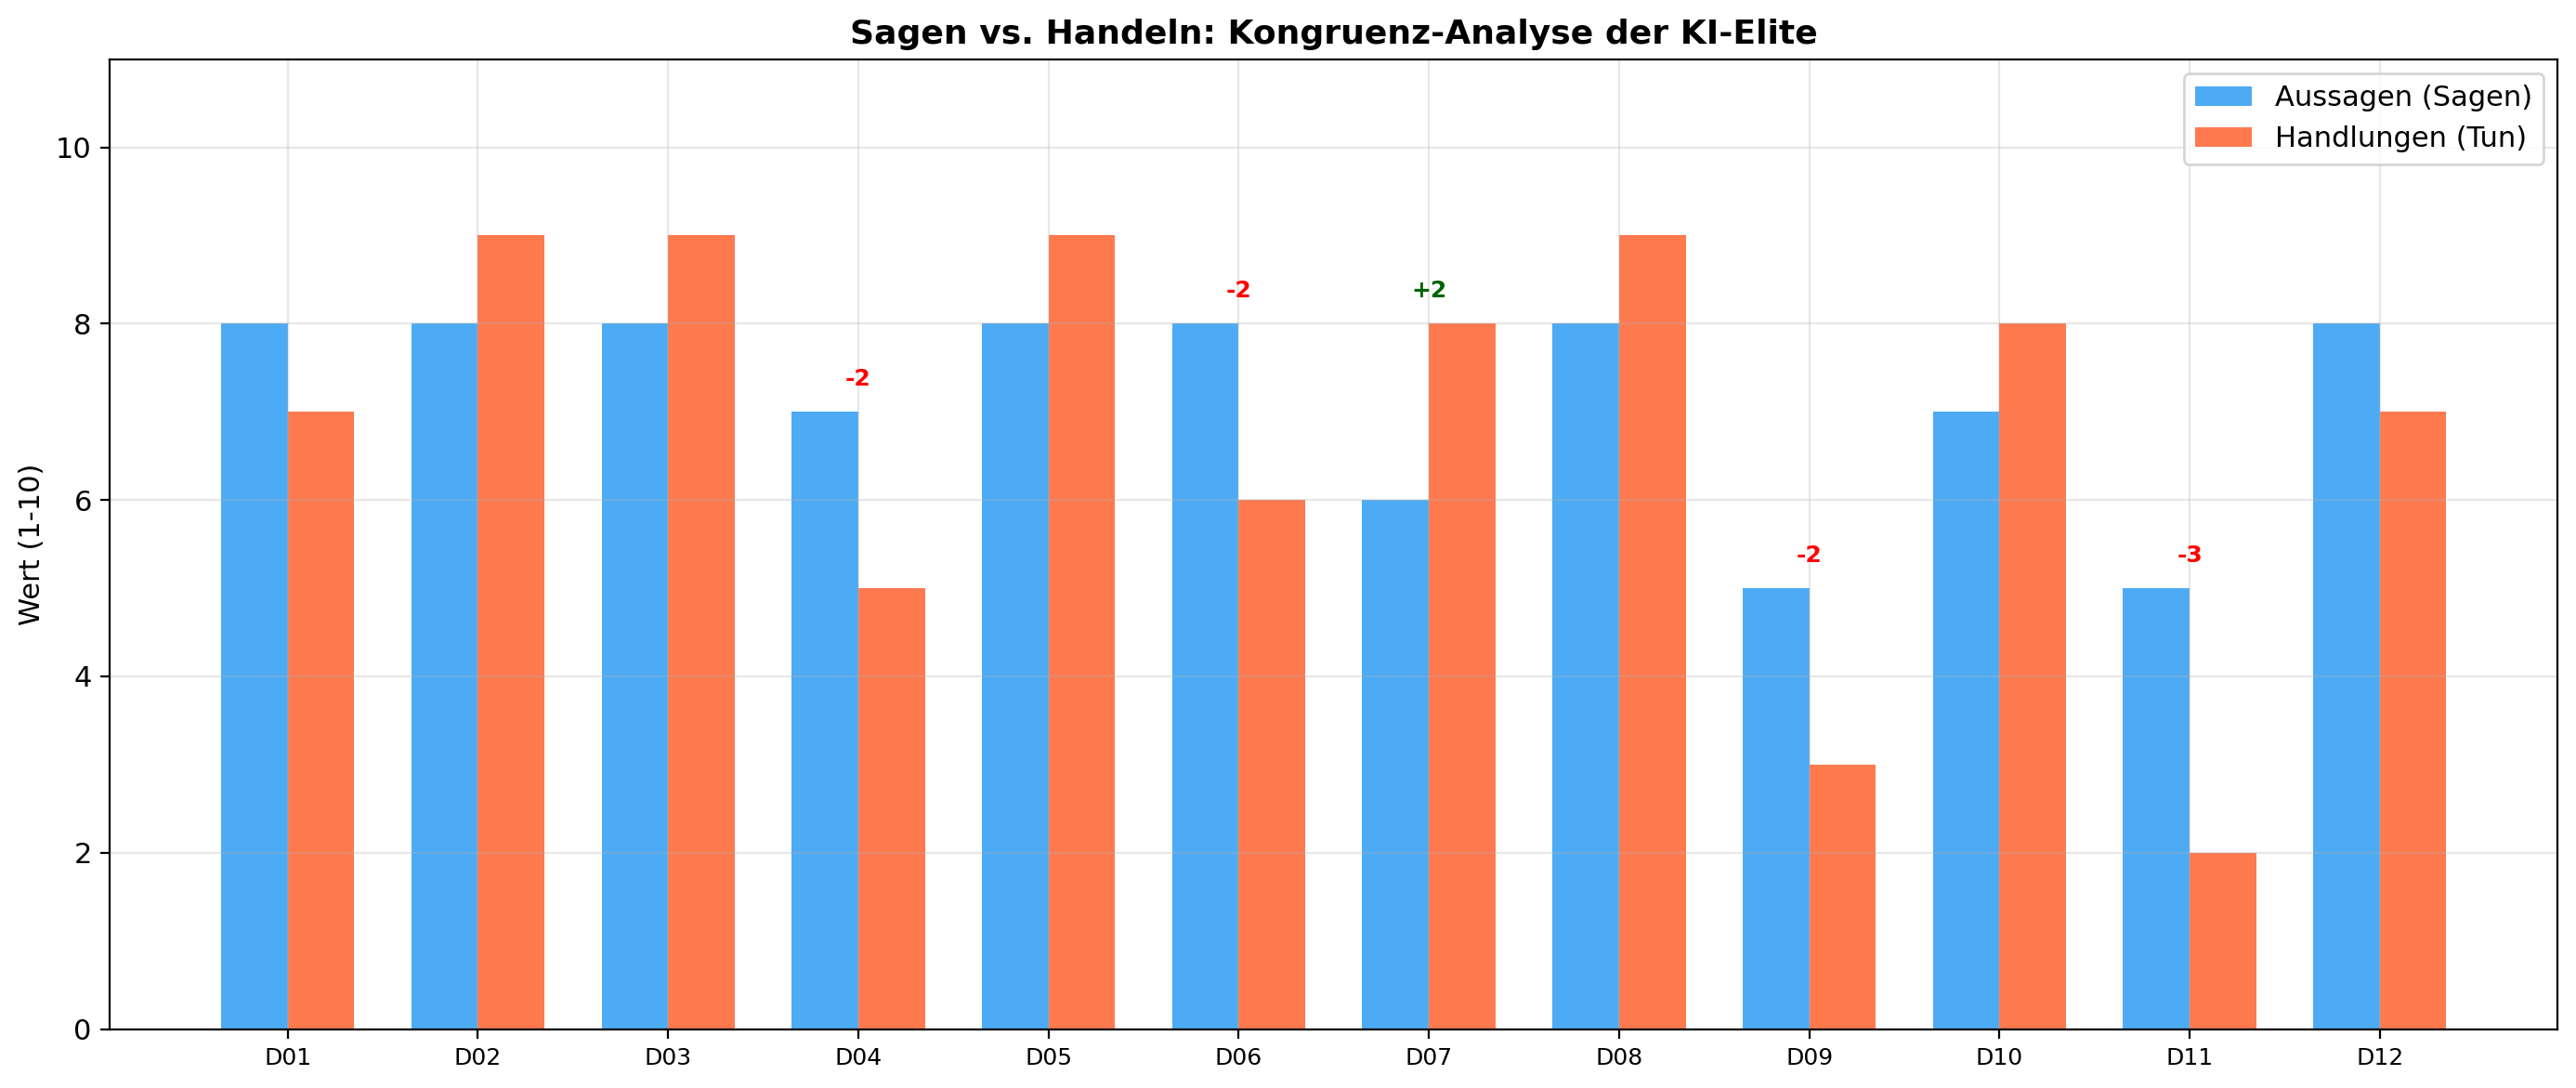
\includegraphics[width=0.95\textwidth]{fig6_sagen_vs_handeln.png}
  \caption{Say vs.\ Do: comparison of worldviews reconstructed from statements (S) and actions (A). The society-oriented dimensions (D04, D06, D09, D11) systematically decline in action, while power-related dimensions (D07, D05) rise.}
  \label{fig:sagen_handeln}
\end{figure}

The largest stable discrepancy (D11, $\Delta\,-2$ in v2, $-3$ in v1) shows: in statements, the AI elite speaks of ``access for all''; in their actions, they build dual-class share structures, concentrate compute infrastructure, and create exclusive networks. D07 (power concentration, $\Delta\,+2$) is the complementary finding: rhetoric favors distributed governance, but operational decisions centralize control.

\medskip
\noindent\textbf{Core finding RQ3:} Two robust say-do discrepancies survive instance separation: D07~(power concentration) and D11~(egalitarianism). The overall gap magnitude is sensitive to measurement conditions and should not be over-interpreted from single runs. But the \emph{direction} of the asymmetry is stable: public discourse is more egalitarian and more power-distributing than operational behavior. Formal quantification (with confidence intervals from $N \geq 30$ repeated measurements) remains a desideratum.


\subsubsection{Group-Level Say-Do Decomposition}

The aggregate say-do comparison masks substantial group-specific variation -- a Simpson's paradox. When five sociological groups are analyzed with strict instance separation (statement corpus and action corpus processed by independent agents), three distinct patterns emerge:

\begin{itemize}
\item \textbf{CEOs} (MAE $= 1.08$, above baseline): The classical desirability gap. Rhetoric is more egalitarian (D11: Say~5, Do~3, $\Delta = -2$) and less power-concentrating (D07: Say~7, Do~9, $\Delta = +2$) than operational behavior. CEOs say the ``right things'' about distributed governance while building dual-class share structures.

\item \textbf{Risk warners} (MAE $= 1.92$, strongest gap): Not an inverse gap but \emph{prophetic consistency}. When decomposed by dependent variable, the pattern becomes clear: DV1 (self-image, D01--D04) shows near-perfect consistency (MAE $= 0.8$) -- risk warners know who they are. The discrepancy concentrates in DV3 (view of humanity, MAE $= 3.2$): their \emph{statements} describe a feared future -- humanity as replaceable (D09: Say~4), posthumanist transformation as inevitable (D10: Say~9) -- while their \emph{actions} reveal their actual values: high human appreciation (D09: Do~8), rejection of posthumanism in practice (D10: Do~4), active agency (D12: Do~8). This is the structure of prophetic warning: articulating a possibility projection one seeks to \emph{prevent}, then acting consistently against it. Their say-do gap is not hypocrisy but the signature of anticipatory ethics -- a finding that would be invisible without the group-level decomposition.

\item \textbf{Investors} (MAE $= 0.75$, below baseline): The most consistent group. Rhetoric and action tell the same story: radical techno-optimism with minimal egalitarian orientation. No desirability gap -- they mean what they say.

\item \textbf{Accelerators} (MAE $= 0.92$, at baseline): A borderline pattern resembling a weaker version of the CEO gap. Rhetoric is more optimistic about progress (D06: $\Delta = -2$), more responsible (D04: $\Delta = -2$), and more egalitarian (D11: $\Delta = -2$) than operational behavior.
\end{itemize}

\noindent These opposing group-level gaps cancel in the aggregate (overall MAE $= 0.75$, below the G6~v2 control baseline of $0.92$). The say-do gap is not absent -- it is \emph{group-specific and directional}, requiring decomposition rather than aggregate reporting.


\subsection{RQ4 -- Worldview Clusters}
\label{sec:ergebnisse:f4}

Four distinct worldview types -- conceived as Weberian ideal types, not as emergent data clusters -- can be identified from the data (Table~\ref{tab:typen}).

\textbf{Identification method:} Cluster identification followed a two-stage procedure. \emph{Stage~1 (LLM-assisted):} All 15 group syntheses were grouped by similarity patterns across the 12~dimensions, with the largest variance axes (D07~power concentration, D09~human appreciation, D11~egalitarianism) serving as discriminating features. \emph{Stage~2 (author validation):} The four-cluster solution proposed by the LLM was evaluated by the author for substantive coherence and plausibility. Alternative solutions (three and five clusters) were examined and rejected: three clusters merge Innovator and Liberator, which is not substantively justified; five clusters split the Guardian type into a subgroup that could not be stably reproduced. We emphasize that this cluster identification is \emph{exploratory} -- a confirmatory validation on an independent dataset is pending. The cluster solution is an \emph{interpretive hypothesis}, not a statistically confirmed result in the sense of formal cluster analysis.

\begin{table}[htbp]
  \centering
  \caption{The four worldview types of the AI elite.}
  \label{tab:typen}
  \small
  \begin{tabular}{l c c c c}
    \toprule
    \textbf{Feature} & \textbf{I ``Architect''} & \textbf{II ``Guardian''} & \textbf{III ``Innovator''} & \textbf{IV ``Liberator''} \\
    \midrule
    $n$ & 35 & 25 & 22 & 18 \\
    Prototype & CEOs, investors & Academics, risk warn. & Founders & Open source \\
    Avg D01--D12 & 7.8 & 6.4 & 7.2 & 6.8 \\
    D04 Responsibility & 6.3 & \textbf{9.0} & 8.3 & 6.0 \\
    D07 Power conc. & \textbf{8.8} & 4.8 & 6.5 & \textbf{2.5} \\
    D09 Human appr. & \textbf{3.3} & 5.8 & 4.8 & \textbf{6.5} \\
    D11 Egalitarianism & \textbf{2.8} & \textbf{7.2} & 5.0 & \textbf{7.5} \\
    \bottomrule
  \end{tabular}
\end{table}

The \textbf{Architect} combines maximal sense of mission with minimal egalitarianism: power concentration is the prerequisite for agency. The \textbf{Guardian} forms the counterpoint: maximal responsibility, demand for institutional constraint. The \textbf{Innovator} occupies a middle position. The \textbf{Liberator} is the most surprising discovery: minimal power concentration \emph{and} high egalitarianism -- anti-regulation actors who want to distribute power more radically than anyone else, albeit through markets and open-source communities.\footnote{The high D11 value of the Liberator type (7.5) marks a construct validity tension: D11 measures orientation toward equality, not its \emph{mechanism}. Market-libertarian access egalitarianism (Liberator) and redistributive egalitarianism (Guardian) produce similar scale values on D11 but mean different things. The exploratory individual-level spot checks (Section~\ref{sec:limitationen:spotchecks}) show that within a cluster type, individual actors can deviate substantially from the cluster mean. Future operationalizations should differentiate here.}

\begin{figure}[htbp]
  \centering
  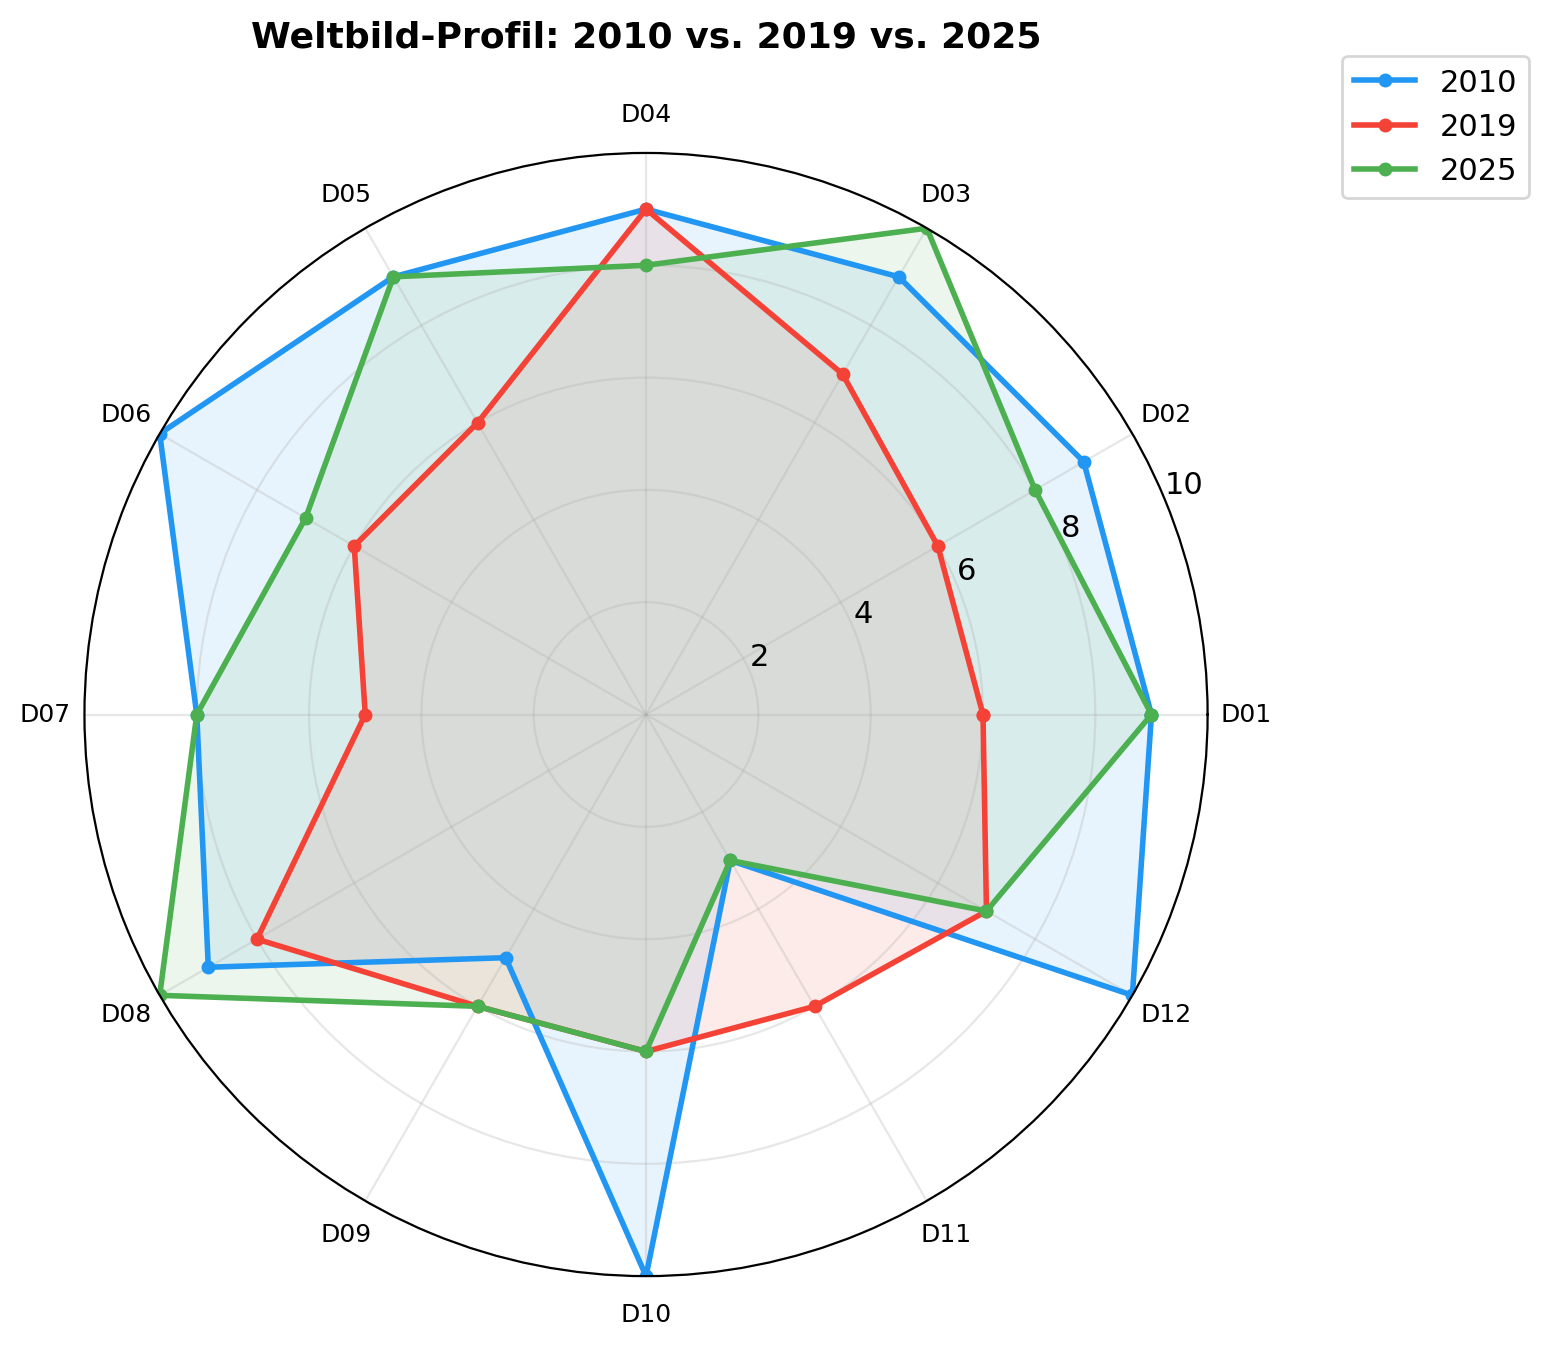
\includegraphics[width=0.85\textwidth]{fig3_radar_vergleich.png}
  \caption{Radar chart of the four worldview types across the 12 dimensions. The polarization between Architect (outer) and Guardian (inner), and the surprising position of the Liberator, are clearly visible.}
  \label{fig:radar}
\end{figure}

\medskip
\noindent\textbf{Core finding RQ4:} The strongest polarization exists between Type~I (logic of domination) and Type~II (logic of participation). The power-moderation paradox -- resource control correlates inversely with egalitarianism and responsibility -- is the finding most critical for democratic theory.


\subsubsection{Algorithmic Structure Check of the Cluster Structure}

To test whether the four worldview types correspond to natural data clusters, we applied HDBSCAN (density-based clustering) and KMeans to the $100 \times 12$ rating matrix. \textbf{HDBSCAN on the full 12-dimensional space} classifies 80--100\% of cases as noise across all parameter configurations tested (\texttt{min\_cluster\_size} $\in \{5, 8, 10, 15\}$, \texttt{min\_samples} $\in \{3, 5\}$); the best-case solution finds only 2~clusters with a negative silhouette score ($-0.15$). KMeans with $k = 4$ yields a silhouette score of only 0.169 -- well below the threshold of 0.25 typically considered indicative of meaningful structure.

\textbf{Subspace clustering}, however, reveals a differentiated picture. On the two strongest discriminating dimensions (D07~power concentration and D11~egalitarianism), HDBSCAN with \texttt{min\_cluster\_size}$\,=5$, \texttt{min\_samples}$\,=2$ identifies 9~clusters with a \emph{silhouette} score of \textbf{0.57} (12\% noise) -- indicating substantial local structure in precisely those dimensions that separate the four ideal types. Similarly, subspace clustering on the three highest-loading PCA dimensions (D02, D05, D09) yields a silhouette of 0.55. We note a circularity caveat: D07 (power concentration) and D11 (egalitarianism) are the same dimensions that define the Architect--Liberator axis in the heuristic typology. The subspace clustering thus partly rediscovers the selection criterion rather than providing independent validation. The result confirms dimensional separability but not the independence of the validation from the typology construction.

This pattern confirms the epistemological status of the four types: they are \textbf{Weberian ideal types} -- heuristic condensations of a multidimensional continuum, not emergent data clusters. Their analytical utility is not diminished by this finding; on the contrary, it is supported by Kruskal-Wallis results across the four types that indicate substantial inter-type differentiation within the reconstructed data (Table~\ref{tab:kruskal}).

\begin{table}[htbp]
  \centering
  \caption{Kruskal-Wallis $H$-test across the four worldview types ($df = 3$, $N = 100$). Significance: {*}{*}{*}\,$p < 0.001$, {*}\,$p < 0.05$, n.s.\,=\,not significant. \textsuperscript{a}Not significant after Bonferroni correction ($\alpha_{\mathrm{adj}} = 0.004$). Note: These tests describe patterns within LLM-generated reconstructions; $p$-values are nominal and should not be interpreted as inferential hypothesis tests in the classical sense.}
  \label{tab:kruskal}
  \footnotesize
  \begin{tabular}{l c c l}
    \toprule
    \textbf{Dimension} & $H$ & $p$ & \textbf{Sig.} \\
    \midrule
    D02 Self-efficacy & 33.55 & $< 0.001$ & {*}{*}{*} \\
    D06 Belief in progress & 29.55 & $< 0.001$ & {*}{*}{*} \\
    D07 Power concentration & 64.76 & $< 0.001$ & {*}{*}{*} \\
    D09 Human appreciation & 17.50 & $< 0.001$ & {*}{*}{*} \\
    D11 Egalitarianism & 49.57 & $< 0.001$ & {*}{*}{*} \\
    D12 Locus of control & 17.93 & $< 0.001$ & {*}{*}{*} \\
    \midrule
    D04 Responsibility & 10.76 & 0.013 & {*}\textsuperscript{a} \\
    D05 Techno-determinism & 11.21 & 0.011 & {*}\textsuperscript{a} \\
    \midrule
    D01 Sense of mission & 2.59 & 0.459 & n.s. \\
    D03 Work ethic & 3.75 & 0.290 & n.s. \\
    D08 Urgency & 6.25 & 0.100 & n.s. \\
    D10 Posthumanism & 4.04 & 0.257 & n.s. \\
    \bottomrule
  \end{tabular}
\end{table}

After Bonferroni correction for 12 simultaneous tests ($\alpha_{\mathrm{adj}} = 0.05/12 = 0.004$), D04 ($p = 0.013$) and D05 ($p = 0.011$) no longer reach significance. The six dimensions with $p < 0.001$ remain significant after correction. Six of twelve dimensions thus show highly significant inter-type differences ($p < 0.001$), while two further dimensions (D04, D05) reach nominal significance at the $p < 0.05$ level but do not survive Bonferroni correction. The four non-significant dimensions (D01, D03, D08, D10) represent the \emph{shared core} of the AI elite worldview -- beliefs on which all four types converge. D07 (power concentration, $H = 64.76$) and D11 (egalitarianism, $H = 49.57$) are the most discriminating dimensions. A circularity caveat applies: since the four types were partly defined \emph{by} D07 and D11, the high $H$-values on these dimensions partly reflect the construction criterion rather than providing independent validation. The Kruskal-Wallis results for the remaining dimensions (D02, D06, D09, D12) are more informative as they were not used in type construction.


\subsection{RQ5 -- Subgroup Comparisons}
\label{sec:ergebnisse:f5}

The inter-group comparisons constitute the analytical core of the study. By systematically comparing the collective worldviews of sociologically defined groups -- differentiated by institutional role, ideological stance, gender, company affiliation, and regulatory position -- the analysis identifies which structural factors are most strongly associated with differences in reconstructed collective belief within the AI elite. Table~\ref{tab:subgruppen} ranks the six most discriminating comparisons.

\begin{table}[htbp]
  \centering
  \caption{Ranking of subgroup differences.}
  \label{tab:subgruppen}
  \small
  \begin{tabular}{c l c c c l}
    \toprule
    \textbf{Rank} & \textbf{Comparison} & \textbf{Avg A} & \textbf{Avg B} & $\Delta$ & \textbf{Strongest contrast} \\
    \midrule
    1 & Risk vs.\ Speed     & 5.9 & 7.6 & 1.7 & D02, D06, D10, D12: each $-5$ \\
    2 & CEOs vs.\ Academics  & 7.8 & 6.3 & 1.5 & D07: $+4$, D11: $-4$ \\
    3 & Women vs.\ Men       & 6.9 & 8.1 & 1.2 & D11: $-6$ \\
    4 & Open vs.\ Closed     & 6.8 & 6.3 & 0.5 & D07: $-3$, D12: $+3$ \\
    5 & Reg-pro vs.\ Contra  & 6.3 & 6.8 & 0.5 & D04: $+4$, D06: $-3$ \\
    6 & Anthropic vs.\ OpenAI & 6.9 & 7.3 & 0.4 & D12: $-3$ \\
    \bottomrule
  \end{tabular}
\end{table}

\begin{figure}[htbp]
  \centering
  
\includegraphics[width=\textwidth]{fig5_gruppen_heatmap.png}
  \caption{Group heatmap: 15 subgroups $\times$ 12 dimensions. The systematic variation of D07 (power concentration) and D11 (egalitarianism) across all comparisons is the central visual finding.}
  \label{fig:gruppen_heatmap}
\end{figure}

The \textbf{strongest contrast} (Risk vs.\ Speed, $\Delta$~1.7) does not concern risk assessment -- both sides estimate catastrophe probability at 10--20\% -- but the ontological pre-commitment: risk warners conceive of AI as a potential autonomous agent, accelerators as a tool.

\textbf{Effect sizes (Cliff's $\delta$)} quantify these contrasts non-parametrically (thresholds following \citealt{Romano2006}: $|\delta| < 0.147$ negligible, $0.147$--$0.33$ small, $0.33$--$0.474$ medium, $> 0.474$ large). The most extreme pairwise differences between the four worldview types emerge on the power-egalitarianism axis: Architect vs.\ Liberator yields $\delta = +1.0$ on D07 (power concentration) and $\delta = -0.98$ on D11 (egalitarianism) -- effectively perfect separation. Architect vs.\ Guardian reaches $\delta = +1.0$ on D07 and $\delta = -0.68$ on D11. Across all six cluster pairs, D07 and D11 each produce five medium-to-large effects ($|\delta| \geq 0.33$), confirming them as the primary discriminating dimensions.

\textbf{Role-based comparisons} show similarly strong effects: Academics vs.\ Investors differ at the \emph{large} level on 9 of 12~dimensions (most strikingly D02~self-efficacy: $\delta = -0.88$; D12~locus of control: $\delta = -0.71$; D09~human appreciation: $\delta = +0.68$). CEOs vs.\ Academics yield large effects on 6~dimensions (D02: $\delta = +0.79$; D06: $\delta = +0.58$; D12: $\delta = +0.55$).

\textbf{Gender differences} reach significance on 7 of 12~dimensions. The largest effects concern D09~human appreciation ($\delta = +0.59$, large: women score higher), D05~techno-determinism ($\delta = -0.50$, large: men score higher), and D11~egalitarianism ($\delta = +0.46$, medium). These effect sizes are more moderate than the nominal group-level contrasts ($\Delta = 6$) would suggest, which is expected: Cliff's $\delta$ captures the full distribution overlap, not just means. The contamination caveat stated above applies with full force.

The \textbf{largest nominal single contrast} in the entire survey is found at D11 in the gender comparison: six full scale points (Women:~8, Men:~2). The female worldview is not an anti-technology worldview but a \emph{conditioned} technology worldview: equally optimistic but with stronger ethical conditions. This finding, however, is the \emph{most contamination-prone} of the entire study and is therefore classified as a \emph{preliminary hypothesis}, not as a confirmed finding. The reasons: (a)~LLMs reproduce known gender stereotypes, especially the attribution of heightened social orientation to women \citep{Santurkar2023}; (b)~the female subsample is small ($n = 18$); (c)~the effect size ($\Delta = 6$) markedly exceeds what comparable empirical studies have observed. An independent validation -- ideally through replication by other research teams using different models and expert ratings -- is particularly urgent for this finding.

The \textbf{biggest surprise} lies in the regulation comparison: anti-regulators have the lowest power concentration value of all 15~groups (D07=2). This contradicts the widespread narrative that anti-regulators represent corporate interests.

\medskip
\noindent\textbf{Core finding RQ5:} The three structural factors most strongly associated with worldview differences in the reconstructed data are ideological stance, institutional role, and gender. The most polarizing dimensions are D11 and D07. The \emph{question of power} is the core of internal differences.


\subsection{RQ6 -- Power and Worldview}
\label{sec:ergebnisse:f6}

\emph{Power} is understood operationally in this study as resource control: the ability to command capital, compute infrastructure, research teams, and political access, and thereby influence the direction of AI development. This definition follows the sociological concept of power in the sense of Weber (``the chance to impose one's own will even against resistance'') and Bourdieu (capital accumulation as a power mechanism), without claiming a comprehensive power-theoretical analysis.

\begin{table}[htbp]
  \centering
  \caption{Worldview types and resource control.}
  \label{tab:macht}
  \begin{tabular}{l c c c l}
    \toprule
    \textbf{Type} & \textbf{Avg} & \textbf{D11} & \textbf{D04} & \textbf{Resources} \\
    \midrule
    I Architect   & 7.8 & 2.8 & 6.3 & Highest \\
    III Innovator & 7.2 & 5.0 & 8.3 & High \\
    IV Liberator  & 6.8 & 7.5 & 6.0 & Medium \\
    II Guardian   & 6.4 & 7.2 & 9.0 & Lowest \\
    \bottomrule
  \end{tabular}
\end{table}

The higher the worldview intensity, the lower the values for human appreciation and egalitarianism, and the higher the acceptance of power concentration. The investor profile marks the extreme case: maximal self-efficacy (D02=10) with minimal sense of responsibility (D04=4) -- ``power without accountability.'' The Top~10 lie exactly one point above the collective on ten of twelve dimensions -- with one decisive exception: human appreciation and egalitarianism lie \emph{below}. Power intensifies all beliefs except those that question power itself.

\medskip
\noindent\textbf{Core finding RQ6:} The reconstructed profiles suggest a correlation between economic power and worldview extremity, combined with an inverse correlation with egalitarianism and responsibility. Since both sides of this observation rest on LLM reconstructions, it remains unclear whether the correlation reflects empirical reality or internal model coherence. If robust, this would be the finding most relevant for democratic theory.


%% =============================================================================
%% SYNOPSIS OF CORE FINDINGS
%% =============================================================================

\begin{table}[htbp]
  \centering
  \caption{Synopsis of the six core findings: result, confidence, and validation status. Confidence classification: \emph{High} = stable across $\geq 3$ group syntheses and supported by inter-group consistency or internal coherence checks; \emph{Medium-high} = stable but without external validation; \emph{Medium} = exploratory, dependent on cluster solution or small subgroup.}
  \label{tab:synopse}
  \footnotesize
  \begin{tabularx}{\textwidth}{l X c c}
    \toprule
    \textbf{RQ} & \textbf{Core finding} & \textbf{Confidence} & \textbf{Ext.\ val.?} \\
    \midrule
    RQ1 & Technological messianism with ambivalence structure (Avg~7.1; dual trough D09/D11) & High & Inter-group \\
    RQ2 & Utopia complex eroding; tragic acceleration compulsion (D10: $-2.4$/dec.) & Medium-high & No \\
    RQ3 & Directional say-do gap (D07 $+2$, D11 $-2$; stable across v1/v2) & Medium & No \\
    RQ4 & Four worldview types: Architect, Guardian, Innovator, Liberator & Medium & No \\
    RQ5 & Strongest predictors: stance, role, gender (preliminary) & Medium & No \\
    RQ6 & Power-moderation paradox: power $\sim$ extremity & High & No \\
    \bottomrule
  \end{tabularx}
\end{table}

%% =============================================================================
%% 5. DISCUSSION
%% =============================================================================
\section{Discussion}
\label{sec:diskussion}

\subsection{Summary and Interpretation}
\label{sec:diskussion:zusammenfassung}

The results \emph{suggest} that the AI elite, analyzed at the group level, holds a \emph{technological messianism with structural ambivalence}. The six research questions coalesce into a coherent picture: RQ1~points to the ``dual trough'' at D09 and D11 as a collective feature; RQ2~suggests an erosion of the utopia complex across epochs; RQ3~indicates directional say-do discrepancies on specific dimensions (D07, D11), though the overall gap magnitude requires cautious interpretation; RQ4~differentiates four worldview types with antagonistic collective positions; RQ5 and RQ6 complete the picture through the power-moderation paradox. The inter-group comparisons (RQ5) constitute the analytical heart of the study: the finding that institutional role, ideological stance, and gender systematically shape collective belief structures carries direct implications for AI governance and democratic theory. All findings are based on LLM-generated group-level reconstructions and should therefore be understood as \emph{empirically supported hypotheses}, not as proven facts. Formulations such as ``shows'' and ``reveals'' are throughout to be read as ``the data suggest.''

Surprising is first the directional consistency of the say-do discrepancies across measurement conditions (D07/D11 stable in v1 and v2); second the retreat of posthumanism (D10 from 10 to 6 -- contradicting the common assumption of increasingly posthumanist orientation); third the existence of the Liberator type (opposition to power concentration also from the libertarian side); fourth the consistency of group-level patterns across multiple independent syntheses.


\subsection{Situating the Findings in the Literature}
\label{sec:diskussion:einordnung}

\citeauthor{Morozov2013}'s solutionism thesis finds nearly complete confirmation (D05=8--9, D06=7--9). However, solutionism is not a monolithic block: risk warners (D05=4) share it substantially less. It is the ideology of the most powerful segment, not of the AI elite as such.

\citeauthor{Daub2020}'s analysis of the philosophical deep structures is confirmed by the narrative syntheses. What the present study adds is the \emph{quantification} and the demonstration that intensity systematically increases with power position.

The Californian Ideology diagnosed by \citet{BarbCam1996} finds its contemporary counterpart in the existence of the Liberator type -- empirically detectable nearly thirty years later.

\citeauthor{Coeckelbergh2020}'s assumption of increasing enhancement orientation is partially \emph{refuted}: the marked decline of posthumanism (D10 from 10 to 6) suggests that the AI elite's interest in the technological transformation of the human being itself has diminished -- in favor of a focus on autonomous AI systems as independent actors.

\emph{On the gender finding.} The extreme contrast at D11 reported in RQ5 (Women:~8, Men:~2, $\Delta = 6$) is the largest single contrast of the entire survey but also the most contamination-prone. LLMs reproduce known gender stereotypes -- especially the attribution of heightened empathy and social orientation to women \citep{Santurkar2023}. Since the female subsample is small ($n = 18$) and the ratings were generated by the same LLM that has internalized these stereotypes, it cannot be distinguished whether the contrast reflects (a)~a real difference in worldviews, (b)~an LLM stereotype artifact, or (c)~a mixture of both. The finding is therefore reported as a \emph{hypothesis} requiring independent validation -- ideally through replication by other research teams using different instruments and expert ratings.

The TESCREAL taxonomy proposed by \citet{TorresGebru2024} (Transhumanism, Extropianism, Singularitarianism, Cosmism, Rationalism, Effective Altruism, Longtermism) finds empirical differentiation in the four-cluster solution: the Architect type embodies the power-political side of the TESCREAL bundle (Singularitarianism, Longtermism), the Guardian type its institutional critique (Effective Altruism with safety focus), the Liberator type the libertarian Extropianism. What the TESCREAL analysis describes as a monolithic ideological bundle appears in the data as a spectrum with at least four distinct positions. \citet{Becker2025} complements this perspective through analysis of the ``broligarchy'' as a social phenomenon: the fusion of technological vision and male power elite, which finds its empirical trace in the gender analysis (RQ5, D11 contrast of 6~scale points).

Paul Ricoeur's ``hermeneutics of suspicion'' \citep{Ricoeur1970} offers a complementary analytical framework: behind the seemingly neutral, technically rational surface of AI elite communication lie power interests and class dynamics that become visible only through systematic deconstruction. The SWR congruence analysis (RQ3) operationalizes this suspicion empirically: the $\Delta$ values between saying and doing show precisely \emph{where} the performative surface diverges from operative reality.

From a sociology-of-science perspective, the decline of egalitarianism (D11) can be read as erosion of Mertonian science norms \citep{Merton1973}: communalism (open access), universalism, and organized skepticism increasingly give way to proprietary, acceleration-centered logics. The transition from research publication to product launch as primary output format is a visible marker of this shift.

The four-cluster solution can furthermore be read through field theory: the antagonistic structure between Architect (economic capital) and Guardian (symbolic capital) reproduces the pattern \citet{Bourdieu1992} diagnosed for the intellectual and artistic field -- an \emph{inverted economic world}. In the AI field: those who control the most resources have the least legitimation through public-interest orientation -- and vice versa. The power-moderation paradox (RQ6) is thus not coincidental but a structural property of the field.

The specific added value compared to essayistic diagnoses lies in three points: \emph{scale} (100 persons, 16 years), \emph{differentiation} (four distinct types), and \emph{validation} (congruence analysis as empirical test).


\subsection{Agentic Alignment vs.\ Worldview Alignment}
\label{sec:diskussion:alignment}

The directional say-do discrepancies indicated by RQ3 (most robust: D07 power concentration $\Delta = +2$, D11 egalitarianism $\Delta = -2$, stable across measurement conditions) can be more precisely captured with a conceptual distinction introduced in this paper, drawing on terminology from the AI alignment debate.\footnote{Neither \emph{Worldview Alignment} nor \emph{Agentic Alignment} as used here corresponds to a fixed established term in the AI alignment literature; the pair is introduced as an analytical heuristic for this study to distinguish the performative from the operative level of value-expression.} \emph{Worldview Alignment} denotes the rhetorical reproduction of desired values -- the public commitment to equality, responsibility, and humanity, as captured by the ``say'' side of the analysis. \emph{Agentic Alignment} denotes actual resource distribution and exercise of power -- the ``do'' side. The findings show that the AI elite exhibits a high degree of Worldview Alignment (the ``right'' values are articulated), while Agentic Alignment systematically deviates. This dualism connects the present AI elite study to the broader alignment debate and raises the question of whether current efforts at ``AI Alignment'' confuse the performative level (Worldview) with the operative one (Agentic).


\subsection{Methodological Reflection}
\label{sec:diskussion:methodik}

The primary achievement of the SWR lies in connecting qualitative depth with quantitative rigor at the group level. The study identifies one reliable instrument -- Claude Opus~4.6, validated through Intra-Model Inter-Instance Rating Reliability (IMIIRR, ICC $= 0.902$) -- and demonstrates its consistent application across all synthesis units. This IMIIRR coefficient exceeds typical human inter-rater reliability in qualitative coding (ICC $= 0.6$--$0.8$; \citealt{Hallgren2012}), and the instrument offers a distinctive advantage over human coders: fully documented prompts replace implicit coding rules, enabling exact replication. The congruence analysis (RQ3) functions as an internal validity test; the stability of the collective profile across 15~group syntheses and 4~types strengthens convergent validity. The inter-group comparisons provide their own form of validation: when different group syntheses -- produced independently from different data subsets -- yield consistent structural patterns (e.g., the D07/D11 axis discriminating across all comparisons), this constitutes evidence for the robustness of the method beyond what any single synthesis could provide. Replication with different frontier models constitutes an independent research task -- analogous to replication of a survey with different interviewer teams -- and is explicitly identified as a desideratum for future work rather than a prerequisite for the present study's validity. The limits of the method -- coherence bias, contamination risk, focus control limits, prompt sensitivity -- are systematically analyzed in the limitations section below (Section~\ref{sec:limitationen}).


\subsection{Societal and Political Implications}
\label{sec:diskussion:implikationen}

The group-level findings carry direct implications for AI governance and democratic theory. The power-moderation paradox -- the systematic finding that institutional groups with the most resources hold collective worldviews furthest from democratic ideals -- poses a concrete challenge for governance architecture. This finding resonates with \citeauthor{Mills1956}'s~(\citeyear{Mills1956}) classic analysis of the ``power elite'' as a self-reinforcing stratum whose worldview diverges systematically from the broader public, and confirms the institutional-economic analysis of \citet{AcemogluJohnson2023}: technological elites tend to steer innovations in ways that reinforce existing power structures rather than break them up -- a pattern the authors trace historically from industrialization to digitalization. Current governance approaches (EU~AI~Act, Executive Order on AI) address the technical artifacts, not the collective worldviews of the groups that produce these artifacts. A complementary approach would need to recognize \emph{epistemic diversity} in AI leadership positions as a regulatory objective.

The systematic group-level say-do gap has a policy implication: voluntary commitments -- currently the preferred form of governance \citep[cf.][]{Bengio2024} -- appear insufficient when entire institutional groups (not just isolated individuals) exhibit consistent discrepancies between public rhetoric and observable action. The findings suggest that binding structural reforms would be more effective than further rounds of voluntary commitments.

The inter-group comparisons reveal a further governance-relevant pattern: the question of power (D07) and equality (D11) is the axis along which all group differences organize. Whether comparing CEOs with academics, accelerationists with risk warners, or men with women -- the power-equality axis is consistently the most discriminating dimension. This suggests that the central ideological fault line within the AI elite is not about technology (all groups are technologically optimistic) but about the \emph{distribution} of technological power.


\subsection{What the Study Does Not Show}
\label{sec:diskussion:negativ}

To prevent frequent misinterpretations, what the present study \emph{does not} accomplish is explicitly stated: (1)~It provides no \emph{causal explanation} for why the AI elite thinks as it does -- that would require biographical case studies, psychological analyses, or historical process analyses. (2)~It does not create \emph{individual profiles} -- the 100~actors serve as data providers; the units of analysis are sociologically defined groups; the ratings are collective group-level abstractions, not personality profiles or individual biographies. (3)~It provides no \emph{predictions} about the future behavior of the AI elite -- the reconstructed worldviews describe the period 2010--2026, not the future. (4)~It does not claim a \emph{representative sample} in the statistical sense -- the 100~individuals were selected by influence, not representativeness. (5)~It does not prove that the \emph{say-do gap} is due to deliberate deception -- alternative explanations (institutional constraints, cognitive dissonance, role-specific communication) are equally plausible.


%% =============================================================================
%% 6. LIMITATIONS
%% =============================================================================
\section{Limitations}
\label{sec:limitationen}

Table~\ref{tab:validation_overview} provides a compact overview of the methodological concerns identified in this study, the countermeasures taken, and their outcomes. The detailed discussion follows in the subsections below.

\begin{table}[htbp]
  \centering
  \caption{Validation overview: methodological concerns, countermeasures, and outcomes.}
  \label{tab:validation_overview}
  \scriptsize
  \begin{tabular}{@{} p{2.4cm} p{1.4cm} p{4.2cm} p{4.5cm} p{1.0cm} @{}}
    \toprule
    \textbf{Concern} & \textbf{Type} & \textbf{Countermeasure} & \textbf{Result} & \textbf{Ref.} \\
    \midrule
    LLM contamination & Design & Focus control (anonymization + task focus) & Variant~C: MAE\,=\,0.67 & QA\,(e) \\[3pt]
    Anthropic circularity & Anticipated & Matched-sample control ($n$\,=\,9 vs.\ 9) & MAE\,=\,1.00, no bias & QA\,(h) \\[3pt]
    Expected-discrepancy & Post hoc & Instance separation (v2 protocol) & Gap $-47\%$; group gaps survive & QA\,(g) \\[3pt]
    Rating instability & Anticipated & IMIIRR ($N$\,=\,15 indep.\ runs) & ICC(3,1)\,=\,0.847, Mean~SD\,=\,0.45 & QA\,(a) \\[3pt]
    Rating order effect & Anticipated & Permutation test (2 orders) & 12/12 identical & QA\,(f) \\[3pt]
    Coherence bias & Anticipated & Outlier detection + inversion control & 80--88\% fit; 58\% $\Delta$\,$\geq$\,5 & QA\,(i,j) \\[3pt]
    Artifactual say-do gap & Anticipated & G6 control corpus & v2 baseline MAE\,=\,0.92 & QA\,(b) \\[3pt]
    Cross-modal validity & Anticipated & Op4 prediction (5 groups) & 72\% confirmed, 0\% contradicted & QA\,(d) \\[3pt]
    Aggregation distortion & Anticipated & Direct vs.\ aggregated comparison & $r$\,=\,0.623, amplification effect & QA\,(c) \\[3pt]
    Influence gradient & Post hoc & Strata comparison (3 rank tiers) & Gradient confirmed; D09/D10 inverse & QA\,(k) \\[3pt]
    Statistical power & Completed & $N$\,=\,15 independent Opus runs & Mean~SD\,=\,0.45; Batch-1 in CI: 3/12 & QA\,(a) \\[3pt]
    Model sensitivity & Desideratum & Inter-model comparison (indep.\ runs) & Future work & \S\,\ref{sec:limitationen} \\
    \bottomrule
  \end{tabular}
\end{table}

\subsection{Data-Related Limitations}

\emph{Source bias.} The data base is limited to public statements and observable actions. The reconstructed worldviews reflect the \emph{publicly presented} worldview, not the \emph{actually held} one. The statement-action comparison (RQ3) offers a partial corrective but cannot eliminate the problem.

\emph{Temporal imbalance.} Data density varies by a factor of ${\sim}43$: from 17~data points in 2010 to 735 in 2024. For 2010--2015, 2--5 statements per person are available; for 2023--2026, 30--80. Criterion K2 (minimum size~15) and documented merging mitigate the problem, and all annual synthesis units meet the minimum threshold; nevertheless, earlier time series rest on thinner evidence and should be interpreted with greater uncertainty.

\emph{Western and language bias.} The sample is disproportionately Anglo-American. Chinese, Japanese, and South Korean AI figures are underrepresented. The findings apply primarily to the Western AI elite.

\emph{Sample dependence.} The selection of the 100~individuals was made by the author using a multi-stage but ultimately subjective scoring procedure. An intersubjective validation of the sample composition (e.g., through independent expert panels) is pending. Since the findings could be sensitive to sample composition, replication with alternative selection procedures is desirable.


\subsection{Methodological Limitations}

\emph{LLM contamination and focus control limits.} Despite consistent focus control, it cannot be excluded that the LLM draws on training knowledge. Focus control operates on two levels: (1)~\emph{anonymization} -- replacing all identifying information with neutral placeholders, ensuring the model cannot anchor on specific individuals -- and (2)~\emph{task focus} -- the prompt design directs the model toward synthesizing a coherent worldview from the presented data without mentioning blinding, identity, or the existence of hidden information (v2~prompts, see repository). An empirical test of the anonymization component confirmed that the choice of blinding strategy (placeholder tokens vs.\ fictional names) has no material effect on group-level ratings ($r = 0.987$, MAE $= 0.33$, max $|\Delta| = 1$; see Section~\ref{sec:methodik:qualitaet}). A third variant (C) tested full identity disclosure -- the same synthesis unit processed with the real names of all group members revealed (Musk, Sutskever, Hinton, Russell, Bengio, Leike). The result showed a moderate but not drastic effect: A--C MAE $= 0.67$, $r = 0.850$, with the same group average (7.1). The largest shift was D11~(egalitarianism, $+2$ points). This confirms that anonymization provides measurable but modest protection; the collective worldview is largely stable even when identities are known. What matters is not whether the model recognizes individuals, but whether it performs its task: constructing a coherent group-level synthesis from the provided data. At the group level, the contamination risk is structurally reduced because no LLM training corpus contains pre-formed collective worldviews of sociological groups.

\emph{Anthropic-internal circularity.} A particularly acute case of the circularity problem concerns the group-level reconstruction of subgroups that include persons directly involved in developing the LLM used. Claude Opus~4.6 is developed by Anthropic; several Anthropic executives (e.g., Dario Amodei, Daniela Amodei) belong to the analyzed sample and their data enter the group-level syntheses. To test for systematic bias, a matched-sample control was conducted: the Anthropic subgroup ($n = 9$) was compared with a matched control group of non-Anthropic founders and researchers ($n = 9$, same size and role composition). The resulting profiles showed MAE $= 1.00$ with no dimension-level difference $|\Delta| \geq 3$. The observed differences -- Anthropic members scoring higher on urgency (D08) and power concentration (D07), the control group higher on posthumanism (D10) and locus of control (D12) -- are interpretable as genuine group differences reflecting Anthropic's safety-focused culture rather than model bias. While this within-model test cannot fully exclude circularity (a cross-model replication remains desirable as external validation), it provides no evidence for systematic Anthropic-specific distortion.

\emph{Expected-discrepancy bias.} The congruence analysis (RQ3) compares two LLM syntheses -- one from statements, one from actions -- both generated by the same model. Since LLMs are trained on social science literature in which say-do discrepancies among elites are a standard finding, an expectation effect is plausible: the model could reproduce the \emph{expected} discrepancy rather than discovering it empirically. This study provides evidence that the effect \emph{exists} but is \emph{controllable}. The original analysis (v1), conducted with both data types in the same LLM instance, produced an aggregate gap of MAE $= 1.42$. When repeated with strict instance separation (v2 protocol) -- each data type processed by an independent agent with no shared context -- the aggregate gap shrank to MAE $= 0.75$ ($-47\%$). This reduction demonstrates that shared context \emph{did} amplify the gap, confirming the expected-discrepancy concern as empirically real. However, the countermeasure (instance separation) is effective: the v2 gap falls below the control baseline (MAE $= 0.92$, from a fictional consistent group processed under matching conditions), indicating that the aggregate gap is no longer reliably distinguishable from measurement noise. The methodologically decisive finding is that \emph{group-specific} gaps survive the correction: CEOs (MAE $= 1.08$) and risk warners (MAE $= 1.92$) both exceed the baseline even under v2 conditions, with stable directional patterns (D07, D11 for CEOs; D09, D10 for risk warners). The expected-discrepancy bias is thus a real methodological concern that was identified, quantified, and partially controlled in this study -- not an unaddressed limitation.

\emph{Critique of synthetic personas.} The growing literature on LLM-generated synthetic personas counsels caution, but the critique must be carefully scoped. \citet{Santurkar2023} shows that LLMs systematically miss the opinions of specific demographic groups and exhibit ``WEIRD'' biases when used as \emph{opinion generators} -- i.e., when prompted to simulate what a demographic group might think. Similarly, \citet{Argyle2023} find that synthetic agents capture key themes but fail at the authentic depth of real discourse when \emph{generating} qualitative data. A recent systematic review of 63 peer-reviewed persona experiments (2023--2025) confirms this pattern: most studies underspecify the target population, only 35\,\% address representativeness, and ecological validity is consistently poor \citep{Batzner2025WhosePersonae}. These critiques target a fundamentally different use case than SWR. In the present study, the LLM does not generate opinions; it \emph{condenses} 3,132 real data points (documented statements and actions) into structured group-level profiles. The synthetic persona is an analytical compression instrument -- closer to the Weberian ideal type than to the simulation agent. The WEIRD bias identified by \citeauthor{Santurkar2023} is largely orthogonal: the AI elite \emph{is} a Western, educated, rich, and industrialized population, so any demographic skew in the model's priors aligns with rather than distorts the target group. Nevertheless, the tendency to overrepresent publicly dominant narratives and underrepresent idiosyncratic or contradictory positions within the group remains a genuine limitation.

\emph{Coherence bias.}\footnote{The term \emph{coherence bias} is used in this study as an operational label; no established concept by this exact name was found in the methodological literature. The underlying phenomenon --- LLMs' tendency to produce logically coherent syntheses that may oversmooth genuine inconsistency in the source data --- is addressed empirically through the deviation detection and inversion controls described in Section~\ref{sec:methodik:qualitaet}.} LLMs are optimized for logical coherence; humans are inherently inconsistent. For worldview reconstruction, this property is both an operational asset and a source of systematic distortion. The asset: coherence enables the SWR to extract a stable, interpretable group-level profile from heterogeneous data -- the method \emph{exploits} coherence as a compression mechanism, analogous to how factor analysis exploits covariance structure. The distortion: the resulting cluster types (Architect, Guardian, Innovator, Liberator) may appear more sharply contoured than they are in reality. Internal tensions that real persons experience -- e.g., between power striving and sense of responsibility -- risk being resolved by the LLM in favor of a consistent profile. The genuine limitation is therefore \emph{over-coherence}: clusters sharper than empirical reality. Two control mechanisms partially address this risk: (1)~the deviation detection built into the SWR pipeline yields group-level fit in the range of 80--88\%, not 100\%, indicating that the model registers and preserves within-group heterogeneity; and (2)~the inversion control (Op3, congruence analysis) shows that 58\% of dimensions exhibit $|\Delta| \geq 5$, demonstrating that the method does not smooth away substantive discrepancies.

\emph{Data bias in say-do reconstruction.} The data available to the SWR method are structurally asymmetric: public statements are abundant and explicit, while actions must be inferred from documented decisions, investments, and organizational behavior. This asymmetry means that the ``say'' side rests on denser evidence than the ``do'' side. The LLM's training corpus reflects this same asymmetry -- public discourse is overrepresented relative to documented operational behavior. This data limitation is particularly relevant for the say-do comparison, where the action profile may be less precisely calibrated than the statement profile. The robust directional gaps (D07 power concentration, D11 egalitarianism) persist across measurement conditions, but their magnitude should be interpreted conservatively given this structural asymmetry. The limitation is inherent in the data structure, not in the method: any analyst -- human or algorithmic -- working from public sources would face the same evidential asymmetry.

\emph{Quantification and internal consistency.} The dimensional correlations reported in Section~\ref{sec:ergebnisse:f2} (e.g., $r_s = +0.85$ between D10 and D12) are generated within the LLM's rating process and could partly reflect internal consistency rather than empirical relationships. This concern applies specifically to the \emph{rating step} (Op2) and is shared by any rating procedure including human raters: a human coder who rates posthumanism high will, by cognitive coherence, also tend to rate locus of control high. The concern does \emph{not} apply to the qualitative syntheses (Op1), which are generated from the raw data without dimensional prompting. Several validation results constrain the scope of this limitation: (1)~the cross-modal prediction (G5, 72\% confirmed) demonstrates that LLM-reconstructed patterns have empirical substance -- predictions derived from statements were confirmed by independently evaluated actions; (2)~the rating order invariance test shows that the ratings do not depend on the sequence of dimensions presented; (3)~the IMIIRR coefficients (ICC $= 0.902$ from $5 \times 2$ runs; ICC $= 0.847$ from $N = 15$ independent single-instance runs) establish that the rating procedure is stable and reproducible. The reported correlations should be read as patterns within a reliably calibrated reconstruction instrument, not as artifacts of arbitrary model behavior -- but external replication remains desirable for confirming which specific correlations hold across instruments.

\emph{Statistical power.} A formal power analysis was conducted on one group-level synthesis unit (GA\_ges\_AH) using $N = 15$ fully independent Opus instances (each a separate agent with no shared context). The results show that the instrument is highly stable: mean SD $= 0.45$ across all 12~dimensions (range: 0.00--0.74), with 95\% confidence intervals narrower than $\pm 0.5$ scale points for most dimensions. The original Batch-1 single measurement fell within only 3 of 12 confidence intervals (MAE to $N = 15$ mean $= 0.73$), confirming that single-run estimates are unreliable and that $N \geq 15$ independent runs are needed for robust profile estimation. However, the analysis was conducted on a single synthesis unit; generalization to all 56~SUs remains a desideratum for future work. The reported $\Delta$ values, correlations, and cluster differences at the group level are descriptive patterns in reconstructed data; interpretation rests on substantive judgment informed by the known measurement precision.

\emph{Reproducibility.} LLM outputs are not fully deterministic even at temperature~0. The original syntheses were generated in single runs per SU. Two post-hoc IMIIRR validations establish reproducibility: (1)~five group-level synthesis units processed twice each yielded ICC $= 0.902$, MAE $= 0.40$ ($\pm 0.2$ scale points); (2)~$N = 15$ fully independent single-instance runs on one synthesis unit yielded ICC(3,1) $= 0.847$, mean SD $= 0.45$, with one dimension (D02) showing perfect agreement across all 15~instances. Both within-instrument reliability estimates exceed typical human inter-rater agreement in qualitative coding (ICC $= 0.6$--$0.8$; \citealt{Hallgren2012}), confirming that the LLM-based instrument offers a \emph{reproducibility advantage} over conventional coding. Whether different models from the same or different providers converge on similar profiles remains an open question --- inter-model comparison with strict independence criteria (separate agent per run, no shared context) is identified as a priority for future replication.


\subsection{Conceptual Limitations}

\emph{Aggregation as design feature.} Collective syntheses level individual variation -- this is the intended function of the method, not a byproduct. The study's research questions (RQ1--RQ6) are formulated at the group level; individual variation is noise relative to this analytical objective, just as individual-level variance is noise in any aggregate analysis (national surveys, industry benchmarks, meta-analyses). The algorithmic structure check (PCA, HDBSCAN; Section~\ref{sec:ergebnisse:f4}) confirms that the individual-level rating matrix exhibits genuine structural variation \emph{prior to} aggregation, indicating that the group-level patterns are compressions of real heterogeneity, not artifacts of uniform input data.

\emph{No causal explanation.} The study identifies \emph{what} the AI elite collectively believes and documents temporal associations (RQ2: longitudinal trends) and structural covariations (RQ5: group differences correlated with role, stance, and gender). It does not establish causal mechanisms. The temporal sequence of worldview shifts (e.g., the decline of egalitarianism coinciding with industry commercialization) and the systematic covariation with structural position (e.g., CEO vs.\ academic profiles) provide plausible associative evidence, but the exclusion of third-variable explanations would require other research designs (longitudinal panel studies, natural experiments, or biographical case analyses).

\emph{Epistemological limits of quantification.} The dimensional ratings (1--10 scale) provide a tractable format for aggregation and comparison, but impose a commensurability assumption that warrants explicit reflection. Complex normative orientations -- such as \emph{locus of control over AI} (D07) or \emph{posthumanism} (D10) -- are multidimensional constructs that do not map cleanly onto a single ordered dimension. The numerical assignment is best understood as an \emph{ordinal compression}: a summary judgment of relative position rather than a measurement of an underlying quantity. Three limitations follow from this. First, interval-level interpretations of rating differences are not warranted; the reported Spearman correlations and rank-based cluster analysis respect this constraint. Second, the assignment of a single value to each dimension implies a degree of \emph{reification}: the abstraction of a multi-stranded discursive orientation into a point on a scale. The qualitative synthesis (Op1) preserves the nuance that the rating (Op2) compresses. Third, the 12~dimensions are conceptually distinct but empirically intercorrelated (e.g., $r_s = +0.85$ for D10--D12); some of this covariation may reflect genuine construct overlap rather than independent empirical relationships. These limitations are inherent in any quantitative worldview research and are not specific to the SWR method; they counsel restraint in fine-grained numerical comparisons while leaving the directional patterns and structural contrasts -- the study's primary claims -- unaffected.

\subsection{Research Ethics Reflection}

The study analyzes public figures based exclusively on publicly accessible data. Two design features substantially mitigate ethical concerns.

\emph{Group-level aggregation as ethical safeguard.} The primary units of analysis are sociologically defined groups, not individuals. Individual data are pooled into group corpora before synthesis; no individual worldview profile is reported as a finding. The reconstructed worldviews describe collective tendencies of roles (CEOs, academics) and stances (accelerationists, risk warners), not the psychology of identifiable persons. This aggregation structurally prevents the attribution of specific beliefs to named individuals.

\emph{Standard legitimation.} The study relies on publicly documented professional statements and actions of public figures whose positions on AI development are of considerable public interest (cf.\ APA Ethical Principles, Standard~8.05). No private or confidential information was collected.

\emph{Residual risk.} For small groups (e.g., company-affiliated subgroups with $n = 3$--5), the aggregation provides weaker anonymization -- a quasi-individual profile may emerge. The three individual spot checks (Section~\ref{sec:limitationen:spotchecks}) are presented as data quality indicators, not as substantive findings. Member checking \citep{SoysalTurkmen2024} remains a desideratum for follow-up research.


\subsection{Individual-Level Analysis (Exploratory)}
\label{sec:limitationen:spotchecks}

The study's substantive findings rest entirely on group-level analyses (RQ1--RQ6). Individual-level SWR is methodologically superfluous for the present purpose -- the original public statements and actions are directly available for any individual. SWR's added value lies exclusively in the group-level synthesis, where it creates collective portraits that do not exist in any single source. The following three spot checks are reported solely as \emph{data quality indicators}: if the underlying individual data produce recognizable, verifiable profiles, this supports the quality of the group-level input. Table~\ref{tab:spotchecks} summarizes the results.

\begin{table}[htbp]
  \centering
  \caption{Exploratory individual-level validation: SWR ratings vs.\ documented positions. These individual-level checks serve as plausibility tests for the underlying data quality; the study's substantive findings rest on the group-level analyses (RQ1--RQ6).}
  \label{tab:spotchecks}
  \footnotesize
  \begin{tabularx}{\textwidth}{l c l c l c l}
    \toprule
    & \multicolumn{2}{c}{\textbf{Sam Altman}} & \multicolumn{2}{c}{\textbf{Geoffrey Hinton}} & \multicolumn{2}{c}{\textbf{Marc Andreessen}} \\
    \textbf{Dim.} & \textbf{R} & \textbf{Status} & \textbf{R} & \textbf{Status} & \textbf{R} & \textbf{Status} \\
    \midrule
    D01 Mission  & 9 & conf. & 7 & conf. & 8 & conf. \\
    D02 Efficacy & 9 & conf. & 5 & conf. & 9 & conf. \\
    D03 Work     & 9 & conf. & 7 & plaus. & 8 & conf. \\
    D04 Respons. & 6 & conf. & 10 & conf. & 4 & conf. \\
    D05 Techno.  & 9 & conf. & 6 & conf. & 9 & conf. \\
    D06 Progress & 8 & conf. & 4 & conf. & 9 & conf. \\
    D07 Power    & 9 & conf. & 4 & conf. & 2 & conf. \\
    D08 Urgency  & 9 & conf. & 10 & conf. & 7 & plaus. \\
    D09 Human ap.& 3 & plaus. & 7 & conf. & 4 & plaus. \\
    D10 Posthum. & 8 & conf. & 5 & conf. & 7 & plaus. \\
    D11 Egalit.  & 3 & conf. & 7 & conf. & 2 & conf. \\
    D12 Control  & 8 & conf. & 3 & conf. & 8 & conf. \\
    \midrule
    \multicolumn{1}{r}{\textit{Confirmed}} & & 10/12 & & 11/12 & & 9/12 \\
    \multicolumn{1}{r}{\textit{Plausible}} & & 2/12 & & 1/12 & & 3/12 \\
    \multicolumn{1}{r}{\textit{Not verif.}} & & 0/12 & & 0/12 & & 0/12 \\
    \bottomrule
  \end{tabularx}
\end{table}

\noindent\textbf{Spot-check methodology.} Each rating was checked against at least two independent, publicly documented sources. \emph{Confirmed} (conf.): rating aligns with documented positions and actions. \emph{Plausible} (plaus.): rating is compatible with known positions but no direct source for the specific manifestation is available. \emph{Not verifiable} (n.v.): rating contradicts documented positions or is not verifiable.

\textbf{Altman (Architect):} D01=9 (confirmed by repeated statements about the ``most important technology in human history,'' Davos 2024, US Congress 2023). D07=9 (confirmed by OpenAI's restructuring from non-profit to capped-profit, dual-class shares). D11=3 (confirmed: despite rhetoric of ``AI for everyone,'' OpenAI has increasingly paywalled access). D09=3 (plausible: no direct statement on human replaceability, but focus on AGI as ``next species'').

\textbf{Hinton (Guardian):} D04=10 (confirmed by resignation from Google 2023 to freely warn about AI risks). D08=10 (confirmed by statement that the probability of existential catastrophe is 10--20\%). D12=3 (confirmed: increasing pessimism, ``I'm not sure we can still control this,'' NYT 2023). D03=7 (plausible: high academic productivity known, but no direct statement on work identification in the Silicon Valley style).

\textbf{Andreessen (Liberator):} D07=2 (confirmed by ``Techno-Optimist Manifesto'' 2023: vehement rejection of government regulation, markets as distribution mechanism). D11=2 (confirmed: explicit rejection of redistribution and egalitarianism in the Manifesto). D04=4 (confirmed: responsibility is attributed to the market, not individual actors). D09=4 (plausible: no direct statement, but instrumental view of human labor in VC context).

\textbf{Overall assessment:} 30 of 36 ratings (83\%) are directly confirmed by public sources, 6 of 36 (17\%) are plausible, none contradicts documented positions. These individual-level spot checks provide plausibility evidence for the data quality underlying the group-level syntheses but do not constitute the primary validation strategy. The study's substantive findings rest on the convergence of multiple independent group syntheses (15~groups, 4~cluster types), not on individual-level accuracy. A systematic external validation by independent experts remains a desideratum for future research.


%% =============================================================================
%% 7. CONCLUSION AND OUTLOOK
%% =============================================================================
\section{Conclusion and Outlook}
\label{sec:fazit}

\subsection{Conclusion}

The study posed the question of what the AI elite thinks -- not as individuals, but as sociologically structured groups -- and has presented an empirically grounded answer. Five overarching insights crystallize:

\emph{First:} The AI elite possesses a coherent, empirically reconstructable collective worldview -- technological messianism, sense of mission, belief in progress -- that is stable across multiple independent group syntheses.

\emph{Second:} This collective worldview is in accelerated transformation. The loss of utopian certainties has led to a \emph{tragic acceleration compulsion}: doubting the future one is building, yet building it anyway.

\emph{Third:} The say-do comparison reveals a Simpson's paradox: the aggregate gap is not reliably distinguishable from measurement noise, but group-specific gaps are substantial and survive instance separation. CEOs exhibit a classical desirability gap (D07~$+2$, D11~$-2$: rhetoric is more egalitarian than operational behavior). Risk warners show an inverse pattern -- prophetic consistency rather than hypocrisy: their statements describe a feared posthumanist future (D10~Say$=$9, D09~Say$=$4), while their actions demonstrate the human-centered values they actually hold (D09~Do$=$8, D10~Do$=$4). Investors are the most consistent group: radical techno-optimism in both word and deed. The say-do analysis is thus not a single-number summary but a \emph{group-specific diagnostic} that reveals qualitatively different types of discrepancy.

\emph{Fourth:} Power is not distributed in a worldview-neutral manner. The inter-group comparisons and the influence strata analysis (Top~10 vs.\ Middle vs.\ Bottom~10) converge on the same finding: the most powerful actors hold the most intense worldviews (avg~7.7 vs.\ 6.4 vs.\ 6.1). Two dimensions show an inverse gradient: human appreciation (D09: Top$=$4, Bottom$=$8) and posthumanism (D10: Top$=$8, Bottom$=$3). The power-equality axis (D07/D11) remains the most discriminating dimension across all group comparisons.

\emph{Fifth:} The SWR has proven to be a capable instrument for group-level worldview analysis that combines qualitative depth with quantitative rigor. The convergence of independently produced group syntheses provides a form of validation specific to the group-level approach. In particular, the decomposition into statement and action profiles (RQ3) proves to be an independent methodological contribution that reveals qualitatively different gap types -- desirability gaps, prophetic consistency, and authentic alignment -- depending on the group's structural position. This diagnostic capability could be transferred beyond the AI elite to political, economic, or military elites.

\subsection{Outlook}

Five directions for future research: (1)~\emph{Comparative extension:} The present study focuses heavily on the US-American, Silicon Valley-centric elite. A central research gap concerns the comparative study of Chinese (Baidu, ByteDance, Alibaba), Indian (Infosys, TCS), and European (Mistral, Aleph Alpha) AI elites. It is unclear whether ``technological messianism'' is a universal artifact of AI development or a specific cultural product of Western libertarianism. Cross-cultural group comparisons (Western vs.\ Chinese vs.\ European AI elites) would test the generalizability of the group-level patterns identified here. (2)~\emph{Finer-grained group analyses:} Expanding the group comparisons to additional sociological categories (generational cohorts, educational backgrounds, geographic origins) and tracking cluster-drift across epochs. (3)~\emph{Methodological development:} Independent replication by other research teams using different frontier models, automated validation procedures, standardized quality criteria for group-level syntheses, and systematic power analysis (the present $N = 15$ validation on one SU should be extended to $N \geq 15$ runs per synthesis unit across all core SUs). (4)~\emph{Transfer:} Financial elite, political elite, military AI elite -- applying the group-comparison framework to other power elites. (5)~\emph{Longitudinal continuation:} Annual worldview monitoring as an instrument of democratic control -- conceivable as a standardized index (analogous to the Democracy Index or AI Readiness Index) that systematically and comparably captures changes in the collective worldviews of AI elite subgroups. The question ``What does the AI elite think?'' is not a one-time question. It is a question that democracies must continuously ask.


%% =============================================================================
%% AI DISCLOSURE
%% =============================================================================
\section*{Disclosure Statement: Use of Artificial Intelligence}

\noindent\textbf{AI Disclosure Level~5 (Extensive).}
In preparing this study, two AI models from Anthropic were used extensively.

\emph{Claude Sonnet~4.5} (model ID: \texttt{claude-sonnet-4-5-20251001}; accessed via API, February 2026; temperature~$= 0$; default system prompt; context window 200k tokens) served as the primary rating engine: all 100~individual-level dimensional ratings (D01--D12) and all group-level synthesis ratings were generated by 9~parallel Sonnet agents.

\emph{Claude Opus~4.6} (model ID: \texttt{claude-opus-4-6}; accessed via Claude Code CLI, February--March 2026; temperature~$= 0$; 1M context window) served as the qualitative analysis engine: group-level syntheses, comparative analyses, statistical processing (PCA, HDBSCAN, Kruskal-Wallis, Cliff's $\delta$), all four post-hoc validation experiments (run-convergence, expected-discrepancy control, aggregation-synthesis comparison, cross-modal prediction), visualization of results, and support in structuring and drafting the manuscript.

No other LLM was used. Research design, research questions, data collection strategy, methodological decisions, interpretation of results, and all substantive conclusions originate from the author. All prompts and model parameters are documented in the repository; a prompt archive is provided in Appendix~\ref{app:prompt}.



%% =============================================================================
%% DATA AVAILABILITY
%% =============================================================================

\section*{Data Availability Statement}

\noindent All data collection scripts, qualitative coding scripts, analysis code, and generated figures are publicly available at: \url{https://github.com/research-line/ai-elite-swr}. The repository contains: data collection scripts, the $100\times12$ rating matrix, HDBSCAN and PCA analysis scripts, prompt templates, and dimensional definitions. The database schema and 85 actor-specific collection scripts enable full reproduction of the data pipeline.

%% =============================================================================
%% BIBLIOGRAPHY (EN)
%% =============================================================================
\newpage

\begin{thebibliography}{99}

\bibitem[Barbrook \& Cameron(1996)]{BarbCam1996}
  Barbrook, R.~\& Cameron, A. (1996).
  The Californian Ideology.
  \textit{Science as Culture}, \textit{6}(1), 44--72.

\bibitem[Bengio et~al.(2024)]{Bengio2024}
  Bengio, Y., Hinton, G.~E.~et~al. (2024).
  Managing extreme AI risks amid rapid progress.
  \textit{Science}, \textit{384}(6698), 842--845.

\bibitem[Berger \& Luckmann(1966)]{BergerLuckmann1966}
  Berger, P.~L.~\& Luckmann, T. (1966).
  \textit{The Social Construction of Reality}.
  Garden City: Doubleday.

\bibitem[Booth(1961)]{Booth1961}
  Booth, W.~C. (1961).
  \textit{The Rhetoric of Fiction}.
  Chicago: University of Chicago Press.

\bibitem[Bostrom(2005)]{Bostrom2005}
  Bostrom, N. (2005).
  A history of transhumanist thought.
  \textit{Journal of Evolution and Technology}, \textit{14}(1), 1--25.

\bibitem[Bostrom(2014)]{Bostrom2014}
  Bostrom, N. (2014).
  \textit{Superintelligence: Paths, Dangers, Strategies}.
  Oxford: Oxford University Press.

\bibitem[Broussard(2018)]{Broussard2018}
  Broussard, M. (2018).
  \textit{Artificial Unintelligence: How Computers Misunderstand the World}.
  Cambridge: MIT Press.

\bibitem[OpenAI(2023)]{OpenAI2023Charter}
  OpenAI (2023).
  Our approach to AI safety.
  \textit{OpenAI Blog}, April~5, 2023.
  \url{https://openai.com/blog/our-approach-to-ai-safety}.

\bibitem[Anthropic(2023)]{AnthropicCoreViews2023}
  Anthropic (2023).
  Core views on AI safety: When, why, what, and how.
  \textit{Anthropic Research Blog}, March~8, 2023.
  \url{https://www.anthropic.com/research/core-views-on-ai-safety}.

\bibitem[Coeckelbergh(2020)]{Coeckelbergh2020}
  Coeckelbergh, M. (2020).
  \textit{AI Ethics}.
  Cambridge: MIT Press.

\bibitem[Daub(2020)]{Daub2020}
  Daub, A. (2020).
  \textit{What Tech Calls Thinking}.
  New York: FSG Originals.

\bibitem[Ge et~al.(2024)]{Ge2024}
  Ge, T.~et~al. (2024).
  Scaling synthetic data creation with 1{,}000{,}000{,}000 personas.
  \textit{arXiv:2406.20094}.

% Geiger2026SWR removed -- Paper B will be written after Paper A submission

\bibitem[Fugard \& Potts(2015)]{FugardPotts2015}
  Fugard, A.~J.~B.~\& Potts, H.~W.~W. (2015).
  Supporting thinking on sample sizes for thematic analyses: A quantitative tool.
  \textit{International Journal of Social Research Methodology}, \textit{18}(6), 669--684.

\bibitem[Guest et~al.(2006)]{Guest2006}
  Guest, G., Bunce, A.~\& Johnson, L. (2006).
  How many interviews are enough? An experiment with data saturation and variability.
  \textit{Field Methods}, \textit{18}(1), 59--82.

\bibitem[Habermas(2001)]{Habermas2001}
  Habermas, J. (2001).
  \textit{Die Zukunft der menschlichen Natur}.
  Frankfurt: Suhrkamp.

\bibitem[Hallgren(2012)]{Hallgren2012}
  Hallgren, K.~A. (2012).
  Computing Inter-Rater Reliability for Observational Data: An Overview and Tutorial.
  \textit{Tutorials in Quantitative Methods for Psychology}, \textit{8}(1), 23--34.

\bibitem[Hayes(2025)]{Hayes2025}
  Hayes, A.~S. (2025).
  `Conversing' With Qualitative Data: Enhancing Qualitative Research Through Large Language Models (LLMs).
  \textit{International Journal of Qualitative Methods}, \textit{24}.

\bibitem[Jara-Ettinger(2019)]{JaraEttinger2019}
  Jara-Ettinger, J. (2019).
  Theory of mind as inverse reinforcement learning.
  \textit{Current Opinion in Behavioral Sciences}, \textit{29}, 105--110.

\bibitem[Kurzweil(2005)]{Kurzweil2005}
  Kurzweil, R. (2005).
  \textit{The Singularity Is Near}.
  New York: Viking.

\bibitem[Lessig(1999)]{Lessig1999}
  Lessig, L. (1999).
  \textit{Code and Other Laws of Cyberspace}.
  New York: Basic Books.

\bibitem[Mannheim(1929)]{Mannheim1929}
  Mannheim, K. (1929).
  \textit{Ideologie und Utopie}.
  Bonn: Cohen.

\bibitem[More(2003)]{More2003}
  More, M. (2003).
  Principles of extropy (version 3.11).
  \textit{Extropy Institute}.

\bibitem[More \& Vita-More(2013)]{MoreVitaMore2013}
  More, M.~\& Vita-More, N. (Eds.) (2013).
  \textit{The Transhumanist Reader}.
  Malden: Wiley-Blackwell.

\bibitem[Morozov(2013)]{Morozov2013}
  Morozov, E. (2013).
  \textit{To Save Everything, Click Here}.
  New York: PublicAffairs.

\bibitem[Ng \& Russell(2000)]{NgRussell2000}
  Ng, A.~Y.~\& Russell, S.~J. (2000).
  Algorithms for inverse reinforcement learning.
  In: \textit{Proc.\ ICML 2000}, 663--670.

\bibitem[Nicmanis \& Spurrier(2025)]{NicmanisSpurrier2025}
  Nicmanis, M.~\& Spurrier, H. (2025).
  Getting Started with Artificial Intelligence Assisted Qualitative Analysis.
  \textit{International Journal of Qualitative Methods}, \textit{24}.

\bibitem[Strauss \& Corbin(1990)]{StraussCorbin1990}
  Strauss, A.~\& Corbin, J. (1990).
  \textit{Basics of Qualitative Research}.
  Newbury Park: Sage.

\bibitem[Tai et~al.(2024)]{Tai2024}
  Tai, R.~et~al. (2024).
  An Examination of the Use of Large Language Models to Aid Analysis of Textual Data.
  \textit{International Journal of Qualitative Methods}, \textit{23}.

\bibitem[Gebru \& Torres(2024)]{TorresGebru2024}
  Gebru, T.~\& Torres, \'E.~P. (2024).
  The TESCREAL bundle: Eugenics and the promise of utopia through AGI.
  \textit{First Monday}, \textit{29}(4).

\bibitem[Turner(2006)]{Turner2006}
  Turner, F. (2006).
  \textit{From Counterculture to Cyberculture}.
  Chicago: University of Chicago Press.

\bibitem[Weber(1904)]{Weber1904}
  Weber, M. (1904).
  Die \glqq Objektivit\"at\grqq{} sozialwissenschaftlicher und sozialpolitischer Erkenntnis.
  \textit{Archiv f\"ur Sozialwissenschaft und Sozialpolitik}, \textit{19}, 22--87.

\bibitem[Crawford(2021)]{Crawford2021}
  Crawford, K. (2021).
  \textit{Atlas of AI: Power, Politics, and the Planetary Costs of Artificial Intelligence}.
  New Haven: Yale University Press.

\bibitem[Zuboff(2019)]{Zuboff2019}
  Zuboff, S. (2019).
  \textit{The Age of Surveillance Capitalism: The Fight for a Human Future at the New Frontier of Power}.
  New York: PublicAffairs.

\bibitem[Floridi(2019)]{Floridi2019}
  Floridi, L. (2019).
  Establishing the Rules for Building Trustworthy AI.
  \textit{Nature Machine Intelligence}, \textit{1}(6), 261--262.

\bibitem[Couldry and Mejias(2019)]{Couldry2019}
  Couldry, N. \& Mejias, U.\,A. (2019).
  \textit{The Costs of Connection: How Data Is Colonizing Human Life and Appropriating It for Capitalism}.
  Stanford: Stanford University Press.

\bibitem[Whittaker(2021)]{Whittaker2021}
  Whittaker, M. (2021).
  The steep cost of capture.
  \textit{Interactions}, \textit{28}(6), 50--55.

\bibitem[Floridi(2023)]{Floridi2023}
  Floridi, L. (2023).
  \textit{The Ethics of Artificial Intelligence: Principles, Challenges, and Opportunities}.
  Oxford: Oxford University Press.

\bibitem[Ornstein et~al.(2025)]{OrnsteinEtAl2025}
  Ornstein, J.~T., Blasingame, E.~N.~\& Truscott, J.~S. (2025).
  How to train your stochastic parrot: Large language models for political texts.
  \textit{Political Science Research and Methods}, \textit{13}(2), 264--281.
  \url{https://doi.org/10.1017/psrm.2024.64}.

\bibitem[Santurkar et~al.(2023)]{Santurkar2023}
  Santurkar, S., Durmus, E., Ladhak, F., Lee, C., Liang, P.~\& Hashimoto, T. (2023).
  Whose opinions do language models reflect?
  In: \textit{Proc.\ ICML 2023}.

\bibitem[Argyle et~al.(2023)]{Argyle2023}
  Argyle, L.~P., Busby, E.~C., Fulda, N., Gubler, J.~R., Rytting, C. \& Wingate, D. (2023).
  Out of One, Many: Using Language Models to Simulate Human Samples.
  \textit{Political Analysis}, 31(3), 337--351.

\bibitem[Batzner et~al.(2025)]{Batzner2025WhosePersonae}
  Batzner, J., Stocker, V., Tang, B., Natarajan, A., Chen, Q., Schmid, S. \& Kasneci, G. (2025).
  Whose Personae? Synthetic Persona Experiments in LLM Research and Pathways to Transparency.
  \textit{Proceedings of the AAAI/ACM Conference on AI, Ethics, and Society}, 8(1), 343--354.
  doi:10.1609/aies.v8i1.36553; arXiv:2512.00461.

\bibitem[Soysal \& T\"urkmen(2024)]{SoysalTurkmen2024}
  Soysal, Y.~\& T\"urkmen, S. (2024).
  Reinterpreting the Member Checking Validation Strategy in Qualitative Research Through the Hermeneutics Lens.
  \textit{Qualitative Inquiry in Education: Theory \& Practice}, \textit{2}(1), 42--63.

\bibitem[Acemoglu \& Johnson(2023)]{AcemogluJohnson2023}
  Acemoglu, D.~\& Johnson, S. (2023).
  \textit{Power and Progress: Our Thousand-Year Struggle Over Technology and Prosperity}.
  New York: PublicAffairs.

\bibitem[Becker(2025)]{Becker2025}
  Becker, A. (2025).
  \textit{More Everything Forever: AI Overlords, Space Empires, and Silicon Valley's Crusade to Control the Fate of Humanity}.
  New York: Basic Books.

\bibitem[Bourdieu(1992)]{Bourdieu1992}
  Bourdieu, P. (1992).
  \textit{Les r\`egles de l'art: Gen\`ese et structure du champ litt\'eraire}.
  Paris: Seuil.
  [Dt.: \textit{Die Regeln der Kunst}, Frankfurt: Suhrkamp, 1999.]

\bibitem[Merton(1973)]{Merton1973}
  Merton, R.~K. (1973).
  \textit{The Sociology of Science: Theoretical and Empirical Investigations}.
  Chicago: University of Chicago Press.

\bibitem[Mills(1956)]{Mills1956}
  Mills, C.~W. (1956).
  \textit{The Power Elite}.
  New York: Oxford University Press.

\bibitem[Ricoeur(1970)]{Ricoeur1970}
  Ricoeur, P. (1970).
  \textit{Freud and Philosophy: An Essay on Interpretation}.
  New Haven: Yale University Press.

\bibitem[Romano et~al.(2006)]{Romano2006}
  Romano, J., Kromrey, J.~D., Coraggio, J.~\& Skowronek, J. (2006).
  Appropriate statistics for ordinal level data: Should we really be using t-test and Cohen's d for evaluating group differences on the NSSE and other surveys?
  \textit{Annual Meeting of the Florida Association of Institutional Research}, 1--33.

\end{thebibliography}



%% =============================================================================
%% APPENDIX (EN)
%% =============================================================================
\newpage
\appendix

\section{Sampling Method for the 100 AI Actors}
\label{app:sampling}

The sample was created through a three-stage procedure: (1)~22 systematic web searches $\to$ 187 candidates; (2)~6-category scoring (market capitalization, key technological positions, discourse power, academic influence, political influence, symbolic status); (3)~reduction to 100 ensuring demographic heterogeneity. The final sample comprises 1,738 statements and 1,394 actions (3,132 data points).


\section{The 12 Rating Dimensions (D01--D12)}
\label{app:dimensionen}

\begin{longtable}{l l l l}
  \toprule
  \textbf{Dim.} & \textbf{Name} & \textbf{Pole 1 (=1)} & \textbf{Pole 10 (=10)} \\
  \midrule
  \endfirsthead
  \toprule
  \textbf{Dim.} & \textbf{Name} & \textbf{Pole 1} & \textbf{Pole 10} \\
  \midrule
  \endhead
  D01 & Sense of mission & No mission & Messianic \\
  D02 & Self-efficacy & Powerless & Omnipotent \\
  D03 & Work ethic & Distance & Total identification \\
  D04 & Sense of responsibility & None & World responsibility \\
  D05 & Techno-determinism & Neutral & Determines everything \\
  D06 & Belief in progress & Decline & Golden future \\
  D07 & Power concentration & Radically distribute & With experts \\
  D08 & Urgency & Relaxed & Existential pressure \\
  D09 & Human appreciation & Replaceable & Unique \\
  D10 & Posthumanism & Human stays & Human becomes more \\
  D11 & Egalitarianism & Inequality natural & Strive for equality \\
  D12 & Locus of control & Pessimism & Full control \\
  \bottomrule
\end{longtable}


\section{Reduction Criteria (K1--K9)}
\label{app:reduktion}

\begin{longtable}{l l p{8cm}}
  \toprule
  \textbf{K} & \textbf{Type} & \textbf{Description} \\
  \midrule
  \endfirsthead
  K1 & obligatory & Research question binding: each SU must be linked to $\geq 1$ research question \\
  K2 & obligatory & Minimum size: $\geq 15$ data points per SU \\
  K3 & obligatory & No redundancy: proper subsets are eliminated \\
  K4 & principle & Modality parsimony: S/A separation only for RQ3 \\
  K5 & principle & Temporal parsimony: annual SUs only for RQ2 \\
  K6 & principle & Group parsimony: only a-priori-justified groups \\
  K7 & principle & Stepwise expansion: core first \\
  K8 & principle & Group-level focus: no individual-person SUs; individuals serve as data providers \\
  K9 & principle & Cluster merging: bottom-up replaces a-priori \\
  \bottomrule
\end{longtable}

\textbf{Balance:} ${\sim}1{,}227$ theoretical SUs $\to$ ${\sim}51$--$56$ core SUs (reduction ${\sim}95$\%).


\section{List of Synthesis Units}
\label{app:se}

The core design comprises 43 predefined plus ${\sim}8$--$13$ emergent synthesis units:

{\small
\begin{longtable}{r l l l}
  \toprule
  \textbf{No} & \textbf{SU-ID} & \textbf{IV combination} & \textbf{RQ} \\
  \midrule
  \endfirsthead
  1 & GA\_ges\_AH & All, SA, Total & RQ1a \\
  2 & GA\_ges\_A & All, S only, Total & RQ3a \\
  3 & GA\_ges\_H & All, A only, Total & RQ3a \\
  4 & T10\_ges\_AH & Top~10, SA, Total & RQ1b \\
  5 & HOM\_haeuf\_A & All, frequently repeated S & RQ1c \\
  6--22 & GA\_YYYY\_AH & All, SA, per year & RQ2a \\
  23--26 & GA\_Epoch\_AH & All, SA, 4~epochs & RQ2b \\
  27--30 & GR\_*\_AH & CEOs, Acad., Inv., Founders & RQ5a \\
  31--33 & GF\_*\_AH & Anthropic, OpenAI, Google & RQ5d \\
  34--39 & GH\_*\_AH & Open/Closed, Risk/Speed, Reg & RQ5b--f \\
  40--41 & GD\_*\_AH & Women, Men & RQ5e \\
  42--43 & KG\_*\_AH & Consistent, Contradictory & RQ3c \\
  \bottomrule
\end{longtable}
}

Additionally: 9 comparison runs (Op6), cross-modal prediction (Op4) for 5 groups (72\% confirmed, 0\% contradicted).


\section{Exemplary Prompt (Op2: Rating)}
\label{app:prompt}

The following prompt illustrates the rating query (Op2) for a group synthesis. All prompts are documented in the repository (\url{https://github.com/research-line/ai-elite-swr}).

\begin{quote}
\small\ttfamily
You receive a collection of anonymized statements and actions from a group of persons in the technology sector. Based on these data, you are to assess the collective worldview of the group on the following 12~dimensions (scale 1--10). Justify each assessment with concrete references to the data points. [Followed by: dimension definitions D01--D12 with scale poles, then the anonymized data corpus.]
\end{quote}

\noindent The complete prompt library including synthesis prompts (Op1), rating prompts (Op2), cross-modal prompts (Op4a/Op4b), and dialogue prompts (Op6) is archived in the repository (\texttt{prompts/en/}). The prompt design rationale follows the focus control principles described in Section~\ref{sec:methodik:qualitaet}.



\end{document}
